\documentclass[10pt,]{article}
\usepackage[left=1in,top=1in,right=1in,bottom=1in]{geometry}
\newcommand*{\authorfont}{\fontfamily{phv}\selectfont}
\usepackage[]{mathpazo}


  \usepackage[T1]{fontenc}
  \usepackage[utf8]{inputenc}




\usepackage{abstract}
\renewcommand{\abstractname}{}    % clear the title
\renewcommand{\absnamepos}{empty} % originally center

\renewenvironment{abstract}
 {{%
    \setlength{\leftmargin}{0mm}
    \setlength{\rightmargin}{\leftmargin}%
  }%
  \relax}
 {\endlist}

\makeatletter
\def\@maketitle{%
  \newpage
%  \null
%  \vskip 2em%
%  \begin{center}%
  \let \footnote \thanks
    {\fontsize{18}{20}\selectfont\raggedright  \setlength{\parindent}{0pt} \@title \par}%
}
%\fi
\makeatother




\setcounter{secnumdepth}{0}

\usepackage{longtable,booktabs}

\usepackage{graphicx,grffile}
\makeatletter
\def\maxwidth{\ifdim\Gin@nat@width>\linewidth\linewidth\else\Gin@nat@width\fi}
\def\maxheight{\ifdim\Gin@nat@height>\textheight\textheight\else\Gin@nat@height\fi}
\makeatother
% Scale images if necessary, so that they will not overflow the page
% margins by default, and it is still possible to overwrite the defaults
% using explicit options in \includegraphics[width, height, ...]{}
\setkeys{Gin}{width=\maxwidth,height=\maxheight,keepaspectratio}


\title{Political Donor Polarization  }



\author{\Large \vspace{0.05in} \newline\normalsize\emph{}  }


\date{}

\usepackage{titlesec}

\titleformat*{\section}{\normalsize\bfseries}
\titleformat*{\subsection}{\normalsize\itshape}
\titleformat*{\subsubsection}{\normalsize\itshape}
\titleformat*{\paragraph}{\normalsize\itshape}
\titleformat*{\subparagraph}{\normalsize\itshape}





\newtheorem{hypothesis}{Hypothesis}
\usepackage{setspace}


% set default figure placement to htbp
\makeatletter
\def\fps@figure{htbp}
\makeatother

\usepackage{graphicx}

% move the hyperref stuff down here, after header-includes, to allow for - \usepackage{hyperref}

\makeatletter
\@ifpackageloaded{hyperref}{}{%
\ifxetex
  \PassOptionsToPackage{hyphens}{url}\usepackage[setpagesize=false, % page size defined by xetex
              unicode=false, % unicode breaks when used with xetex
              xetex]{hyperref}
\else
  \PassOptionsToPackage{hyphens}{url}\usepackage[draft,unicode=true]{hyperref}
\fi
}

\@ifpackageloaded{color}{
    \PassOptionsToPackage{usenames,dvipsnames}{color}
}{%
    \usepackage[usenames,dvipsnames]{color}
}
\makeatother
\hypersetup{breaklinks=true,
            bookmarks=true,
            pdfauthor={ ()},
             pdfkeywords = {},  
            pdftitle={Political Donor Polarization},
            colorlinks=true,
            citecolor=blue,
            urlcolor=blue,
            linkcolor=magenta,
            pdfborder={0 0 0}}
\urlstyle{same}  % don't use monospace font for urls

% Add an option for endnotes. -----


% add tightlist ----------
\providecommand{\tightlist}{%
\setlength{\itemsep}{0pt}\setlength{\parskip}{0pt}}

% add some other packages ----------

% \usepackage{multicol}
% This should regulate where figures float
% See: https://tex.stackexchange.com/questions/2275/keeping-tables-figures-close-to-where-they-are-mentioned
\usepackage[section]{placeins}


\begin{document}
	
% \pagenumbering{arabic}% resets `page` counter to 1 
%
% \maketitle

{% \usefont{T1}{pnc}{m}{n}
\setlength{\parindent}{0pt}
\thispagestyle{plain}
{\fontsize{18}{20}\selectfont\raggedright 
\maketitle  % title \par  

}

{
   \vskip 13.5pt\relax \normalsize\fontsize{11}{12} 
\textbf{\authorfont } \hskip 15pt \emph{\small }   

}

}






\vskip -8.5pt


 % removetitleabstract

\noindent \doublespacing 

\newpage

\hypertarget{testing-difference-in-mean-partisanship-by-geography}{%
\subsection{Testing Difference in Mean Partisanship by
Geography}\label{testing-difference-in-mean-partisanship-by-geography}}

\begin{longtable}[]{@{}llrll@{}}
\caption{Bootstrapped difference-in-means test with 1,000 replications
comparing mean partisanship by geographic category.}\tabularnewline
\toprule
\begin{minipage}[b]{0.34\columnwidth}\raggedright
Geographic Category\strut
\end{minipage} & \begin{minipage}[b]{0.21\columnwidth}\raggedright
Election Year\strut
\end{minipage} & \begin{minipage}[b]{0.09\columnwidth}\raggedleft
Diff.\strut
\end{minipage} & \begin{minipage}[b]{0.16\columnwidth}\raggedright
CI\strut
\end{minipage} & \begin{minipage}[b]{0.06\columnwidth}\raggedright
p\strut
\end{minipage}\tabularnewline
\midrule
\endfirsthead
\toprule
\begin{minipage}[b]{0.34\columnwidth}\raggedright
Geographic Category\strut
\end{minipage} & \begin{minipage}[b]{0.21\columnwidth}\raggedright
Election Year\strut
\end{minipage} & \begin{minipage}[b]{0.09\columnwidth}\raggedleft
Diff.\strut
\end{minipage} & \begin{minipage}[b]{0.16\columnwidth}\raggedright
CI\strut
\end{minipage} & \begin{minipage}[b]{0.06\columnwidth}\raggedright
p\strut
\end{minipage}\tabularnewline
\midrule
\endhead
\begin{minipage}[t]{0.34\columnwidth}\raggedright
1. Urban: Madison \& Milwaukee\strut
\end{minipage} & \begin{minipage}[t]{0.21\columnwidth}\raggedright
2012 compared to 2010\strut
\end{minipage} & \begin{minipage}[t]{0.09\columnwidth}\raggedleft
0.02757\strut
\end{minipage} & \begin{minipage}[t]{0.16\columnwidth}\raggedright
0.02368-0.03127\strut
\end{minipage} & \begin{minipage}[t]{0.06\columnwidth}\raggedright
\textless.001\strut
\end{minipage}\tabularnewline
\begin{minipage}[t]{0.34\columnwidth}\raggedright
2. Urban: Not Madison or Milwaukee\strut
\end{minipage} & \begin{minipage}[t]{0.21\columnwidth}\raggedright
2012 compared to 2010\strut
\end{minipage} & \begin{minipage}[t]{0.09\columnwidth}\raggedleft
0.03453\strut
\end{minipage} & \begin{minipage}[t]{0.16\columnwidth}\raggedright
0.03231-0.0367\strut
\end{minipage} & \begin{minipage}[t]{0.06\columnwidth}\raggedright
\textless.001\strut
\end{minipage}\tabularnewline
\begin{minipage}[t]{0.34\columnwidth}\raggedright
3. Suburban\strut
\end{minipage} & \begin{minipage}[t]{0.21\columnwidth}\raggedright
2012 compared to 2010\strut
\end{minipage} & \begin{minipage}[t]{0.09\columnwidth}\raggedleft
0.03384\strut
\end{minipage} & \begin{minipage}[t]{0.16\columnwidth}\raggedright
0.03046-0.03722\strut
\end{minipage} & \begin{minipage}[t]{0.06\columnwidth}\raggedright
\textless.001\strut
\end{minipage}\tabularnewline
\begin{minipage}[t]{0.34\columnwidth}\raggedright
4. Rural\strut
\end{minipage} & \begin{minipage}[t]{0.21\columnwidth}\raggedright
2012 compared to 2010\strut
\end{minipage} & \begin{minipage}[t]{0.09\columnwidth}\raggedleft
0.04616\strut
\end{minipage} & \begin{minipage}[t]{0.16\columnwidth}\raggedright
0.03915-0.05317\strut
\end{minipage} & \begin{minipage}[t]{0.06\columnwidth}\raggedright
\textless.001\strut
\end{minipage}\tabularnewline
\begin{minipage}[t]{0.34\columnwidth}\raggedright
1. Urban: Madison \& Milwaukee\strut
\end{minipage} & \begin{minipage}[t]{0.21\columnwidth}\raggedright
2014 compared to 2012\strut
\end{minipage} & \begin{minipage}[t]{0.09\columnwidth}\raggedleft
0.00127\strut
\end{minipage} & \begin{minipage}[t]{0.16\columnwidth}\raggedright
-0.00121-0.00392\strut
\end{minipage} & \begin{minipage}[t]{0.06\columnwidth}\raggedright
0.294\strut
\end{minipage}\tabularnewline
\begin{minipage}[t]{0.34\columnwidth}\raggedright
2. Urban: Not Madison or Milwaukee\strut
\end{minipage} & \begin{minipage}[t]{0.21\columnwidth}\raggedright
2014 compared to 2012\strut
\end{minipage} & \begin{minipage}[t]{0.09\columnwidth}\raggedleft
0.00126\strut
\end{minipage} & \begin{minipage}[t]{0.16\columnwidth}\raggedright
0.00016-0.00241\strut
\end{minipage} & \begin{minipage}[t]{0.06\columnwidth}\raggedright
0.03\strut
\end{minipage}\tabularnewline
\begin{minipage}[t]{0.34\columnwidth}\raggedright
3. Suburban\strut
\end{minipage} & \begin{minipage}[t]{0.21\columnwidth}\raggedright
2014 compared to 2012\strut
\end{minipage} & \begin{minipage}[t]{0.09\columnwidth}\raggedleft
-0.00086\strut
\end{minipage} & \begin{minipage}[t]{0.16\columnwidth}\raggedright
-0.0027-0.00104\strut
\end{minipage} & \begin{minipage}[t]{0.06\columnwidth}\raggedright
0.376\strut
\end{minipage}\tabularnewline
\begin{minipage}[t]{0.34\columnwidth}\raggedright
4. Rural\strut
\end{minipage} & \begin{minipage}[t]{0.21\columnwidth}\raggedright
2014 compared to 2012\strut
\end{minipage} & \begin{minipage}[t]{0.09\columnwidth}\raggedleft
0.00288\strut
\end{minipage} & \begin{minipage}[t]{0.16\columnwidth}\raggedright
7e-05-0.00548\strut
\end{minipage} & \begin{minipage}[t]{0.06\columnwidth}\raggedright
0.044\strut
\end{minipage}\tabularnewline
\bottomrule
\end{longtable}

\begin{verbatim}
## Saving 6.5 x 4.5 in image
\end{verbatim}

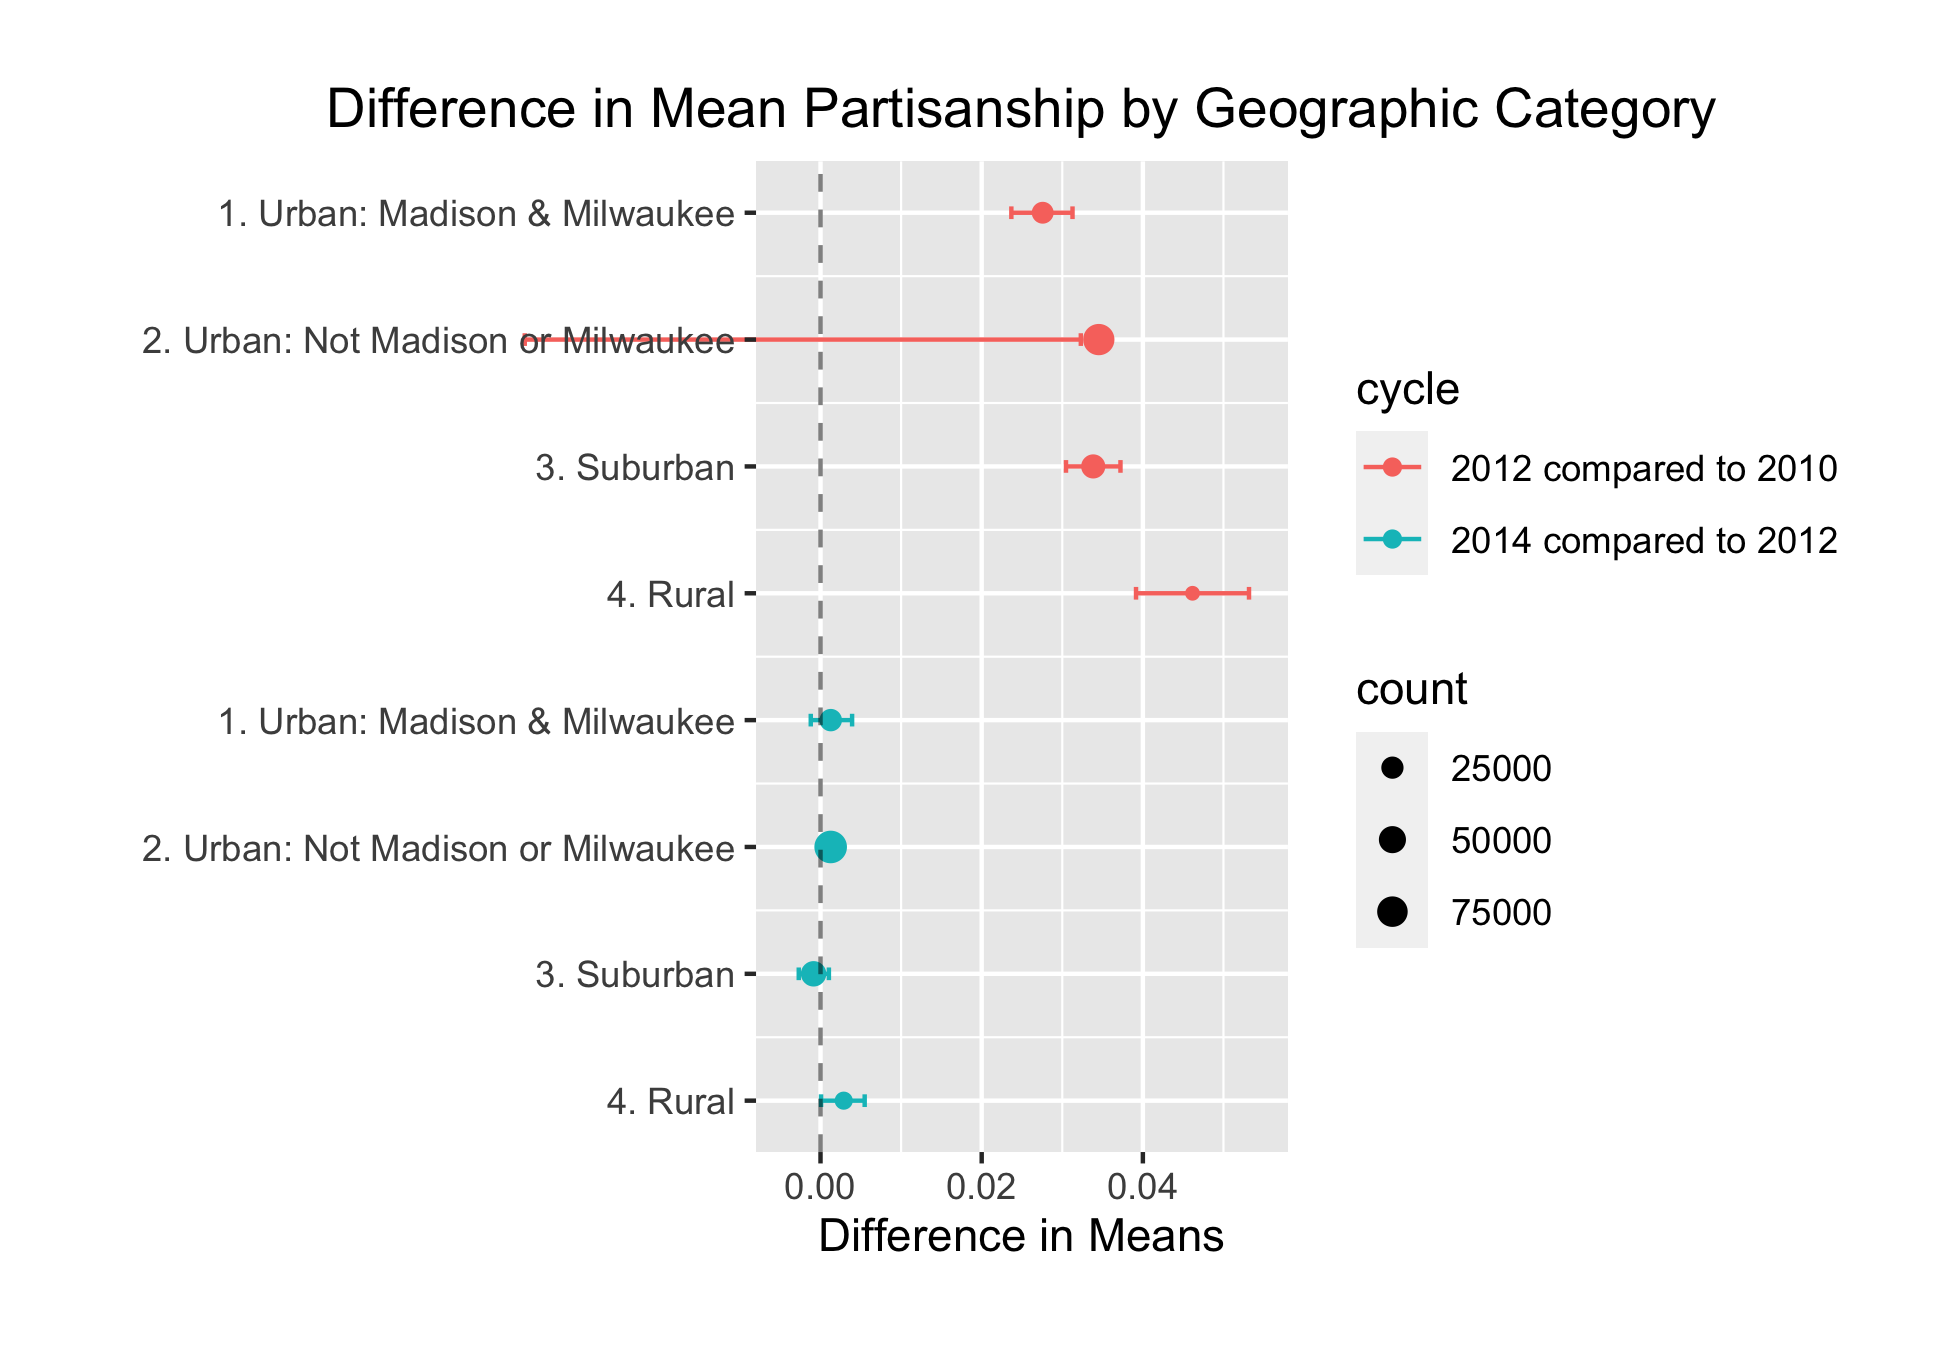
\includegraphics{geo_categories.png}

I grouped the donors according the four geographic categories to run the
same difference-in-means test. The summary statistics tells a story that
largely agrees with the results for the statewide analysis in Table 2;
Wisconsin donors significantly polarized in the 2012 election cycle
across both metropolitan and nonmetropolitan areas and remained that way
come the 2014 election cycle. These results may spark the question:
should we consider donor geography when looking at polarization? The
answer may be rooted in what Cramer describes as ``rural
consciousness,'' or the strong sense of identity that the rural
Wisconsinites felt alongside resentment towards the two main cities in a
rising right-wing populist movement. The people outside of Madison and
Milwaukee resonated with Scott Walker's appeal to their sense of
distributive power injustice which was reflected in Act 10's attack on
public employee unions. Indeed we can look at rural Wisconsin as well as
cities excluding Madison and Milwaukee, which encompass the majority of
Wisconsin's population. These two geographic categories had the greatest
increase in polarization in both election cycles and were significant in
both years. This confirms continuing support for Scott Walker and
reflects the rural consciousness that continued to grow even after the
2012 election.

\newpage

\hypertarget{further-testing-by-party}{%
\subsection{Further Testing by Party}\label{further-testing-by-party}}

\begin{longtable}[]{@{}lllrll@{}}
\caption{Bootstrapped difference-in-means test with 1,000 replications
comparing mean partisanship by geographic category.}\tabularnewline
\toprule
\begin{minipage}[b]{0.29\columnwidth}\raggedright
Geographic Category\strut
\end{minipage} & \begin{minipage}[b]{0.09\columnwidth}\raggedright
Party\strut
\end{minipage} & \begin{minipage}[b]{0.18\columnwidth}\raggedright
Election Year\strut
\end{minipage} & \begin{minipage}[b]{0.07\columnwidth}\raggedleft
Diff.\strut
\end{minipage} & \begin{minipage}[b]{0.14\columnwidth}\raggedright
CI\strut
\end{minipage} & \begin{minipage}[b]{0.05\columnwidth}\raggedright
p\strut
\end{minipage}\tabularnewline
\midrule
\endfirsthead
\toprule
\begin{minipage}[b]{0.29\columnwidth}\raggedright
Geographic Category\strut
\end{minipage} & \begin{minipage}[b]{0.09\columnwidth}\raggedright
Party\strut
\end{minipage} & \begin{minipage}[b]{0.18\columnwidth}\raggedright
Election Year\strut
\end{minipage} & \begin{minipage}[b]{0.07\columnwidth}\raggedleft
Diff.\strut
\end{minipage} & \begin{minipage}[b]{0.14\columnwidth}\raggedright
CI\strut
\end{minipage} & \begin{minipage}[b]{0.05\columnwidth}\raggedright
p\strut
\end{minipage}\tabularnewline
\midrule
\endhead
\begin{minipage}[t]{0.29\columnwidth}\raggedright
1. Urban: Madison \& Milwaukee\strut
\end{minipage} & \begin{minipage}[t]{0.09\columnwidth}\raggedright
democrat\strut
\end{minipage} & \begin{minipage}[t]{0.18\columnwidth}\raggedright
2012 compared to 2010\strut
\end{minipage} & \begin{minipage}[t]{0.07\columnwidth}\raggedleft
0.02734\strut
\end{minipage} & \begin{minipage}[t]{0.14\columnwidth}\raggedright
0.02287-0.03211\strut
\end{minipage} & \begin{minipage}[t]{0.05\columnwidth}\raggedright
\textless.001\strut
\end{minipage}\tabularnewline
\begin{minipage}[t]{0.29\columnwidth}\raggedright
2. Urban: Not Madison or Milwaukee\strut
\end{minipage} & \begin{minipage}[t]{0.09\columnwidth}\raggedright
democrat\strut
\end{minipage} & \begin{minipage}[t]{0.18\columnwidth}\raggedright
2012 compared to 2010\strut
\end{minipage} & \begin{minipage}[t]{0.07\columnwidth}\raggedleft
0.04954\strut
\end{minipage} & \begin{minipage}[t]{0.14\columnwidth}\raggedright
0.04495-0.05416\strut
\end{minipage} & \begin{minipage}[t]{0.05\columnwidth}\raggedright
\textless.001\strut
\end{minipage}\tabularnewline
\begin{minipage}[t]{0.29\columnwidth}\raggedright
3. Suburban\strut
\end{minipage} & \begin{minipage}[t]{0.09\columnwidth}\raggedright
democrat\strut
\end{minipage} & \begin{minipage}[t]{0.18\columnwidth}\raggedright
2012 compared to 2010\strut
\end{minipage} & \begin{minipage}[t]{0.07\columnwidth}\raggedleft
0.04586\strut
\end{minipage} & \begin{minipage}[t]{0.14\columnwidth}\raggedright
0.03958-0.05236\strut
\end{minipage} & \begin{minipage}[t]{0.05\columnwidth}\raggedright
\textless.001\strut
\end{minipage}\tabularnewline
\begin{minipage}[t]{0.29\columnwidth}\raggedright
4. Rural\strut
\end{minipage} & \begin{minipage}[t]{0.09\columnwidth}\raggedright
democrat\strut
\end{minipage} & \begin{minipage}[t]{0.18\columnwidth}\raggedright
2012 compared to 2010\strut
\end{minipage} & \begin{minipage}[t]{0.07\columnwidth}\raggedleft
0.04037\strut
\end{minipage} & \begin{minipage}[t]{0.14\columnwidth}\raggedright
0.03131-0.05044\strut
\end{minipage} & \begin{minipage}[t]{0.05\columnwidth}\raggedright
\textless.001\strut
\end{minipage}\tabularnewline
\begin{minipage}[t]{0.29\columnwidth}\raggedright
1. Urban: Madison \& Milwaukee\strut
\end{minipage} & \begin{minipage}[t]{0.09\columnwidth}\raggedright
democrat\strut
\end{minipage} & \begin{minipage}[t]{0.18\columnwidth}\raggedright
2014 compared to 2012\strut
\end{minipage} & \begin{minipage}[t]{0.07\columnwidth}\raggedleft
0.00135\strut
\end{minipage} & \begin{minipage}[t]{0.14\columnwidth}\raggedright
-0.00073-0.00342\strut
\end{minipage} & \begin{minipage}[t]{0.05\columnwidth}\raggedright
0.22\strut
\end{minipage}\tabularnewline
\begin{minipage}[t]{0.29\columnwidth}\raggedright
2. Urban: Not Madison or Milwaukee\strut
\end{minipage} & \begin{minipage}[t]{0.09\columnwidth}\raggedright
democrat\strut
\end{minipage} & \begin{minipage}[t]{0.18\columnwidth}\raggedright
2014 compared to 2012\strut
\end{minipage} & \begin{minipage}[t]{0.07\columnwidth}\raggedleft
0.00436\strut
\end{minipage} & \begin{minipage}[t]{0.14\columnwidth}\raggedright
0.0024-0.00624\strut
\end{minipage} & \begin{minipage}[t]{0.05\columnwidth}\raggedright
\textless.001\strut
\end{minipage}\tabularnewline
\begin{minipage}[t]{0.29\columnwidth}\raggedright
3. Suburban\strut
\end{minipage} & \begin{minipage}[t]{0.09\columnwidth}\raggedright
democrat\strut
\end{minipage} & \begin{minipage}[t]{0.18\columnwidth}\raggedright
2014 compared to 2012\strut
\end{minipage} & \begin{minipage}[t]{0.07\columnwidth}\raggedleft
-0.00005\strut
\end{minipage} & \begin{minipage}[t]{0.14\columnwidth}\raggedright
-0.00269-0.00269\strut
\end{minipage} & \begin{minipage}[t]{0.05\columnwidth}\raggedright
0.944\strut
\end{minipage}\tabularnewline
\begin{minipage}[t]{0.29\columnwidth}\raggedright
4. Rural\strut
\end{minipage} & \begin{minipage}[t]{0.09\columnwidth}\raggedright
democrat\strut
\end{minipage} & \begin{minipage}[t]{0.18\columnwidth}\raggedright
2014 compared to 2012\strut
\end{minipage} & \begin{minipage}[t]{0.07\columnwidth}\raggedleft
-0.00180\strut
\end{minipage} & \begin{minipage}[t]{0.14\columnwidth}\raggedright
-0.00504-0.00106\strut
\end{minipage} & \begin{minipage}[t]{0.05\columnwidth}\raggedright
0.236\strut
\end{minipage}\tabularnewline
\begin{minipage}[t]{0.29\columnwidth}\raggedright
1. Urban: Madison \& Milwaukee\strut
\end{minipage} & \begin{minipage}[t]{0.09\columnwidth}\raggedright
republican\strut
\end{minipage} & \begin{minipage}[t]{0.18\columnwidth}\raggedright
2012 compared to 2010\strut
\end{minipage} & \begin{minipage}[t]{0.07\columnwidth}\raggedleft
0.01374\strut
\end{minipage} & \begin{minipage}[t]{0.14\columnwidth}\raggedright
0.00833-0.0192\strut
\end{minipage} & \begin{minipage}[t]{0.05\columnwidth}\raggedright
\textless.001\strut
\end{minipage}\tabularnewline
\begin{minipage}[t]{0.29\columnwidth}\raggedright
2. Urban: Not Madison or Milwaukee\strut
\end{minipage} & \begin{minipage}[t]{0.09\columnwidth}\raggedright
republican\strut
\end{minipage} & \begin{minipage}[t]{0.18\columnwidth}\raggedright
2012 compared to 2010\strut
\end{minipage} & \begin{minipage}[t]{0.07\columnwidth}\raggedleft
0.02125\strut
\end{minipage} & \begin{minipage}[t]{0.14\columnwidth}\raggedright
0.0193-0.02315\strut
\end{minipage} & \begin{minipage}[t]{0.05\columnwidth}\raggedright
\textless.001\strut
\end{minipage}\tabularnewline
\begin{minipage}[t]{0.29\columnwidth}\raggedright
3. Suburban\strut
\end{minipage} & \begin{minipage}[t]{0.09\columnwidth}\raggedright
republican\strut
\end{minipage} & \begin{minipage}[t]{0.18\columnwidth}\raggedright
2012 compared to 2010\strut
\end{minipage} & \begin{minipage}[t]{0.07\columnwidth}\raggedleft
0.02013\strut
\end{minipage} & \begin{minipage}[t]{0.14\columnwidth}\raggedright
0.01706-0.02323\strut
\end{minipage} & \begin{minipage}[t]{0.05\columnwidth}\raggedright
\textless.001\strut
\end{minipage}\tabularnewline
\begin{minipage}[t]{0.29\columnwidth}\raggedright
4. Rural\strut
\end{minipage} & \begin{minipage}[t]{0.09\columnwidth}\raggedright
republican\strut
\end{minipage} & \begin{minipage}[t]{0.18\columnwidth}\raggedright
2012 compared to 2010\strut
\end{minipage} & \begin{minipage}[t]{0.07\columnwidth}\raggedleft
0.03207\strut
\end{minipage} & \begin{minipage}[t]{0.14\columnwidth}\raggedright
0.02562-0.03889\strut
\end{minipage} & \begin{minipage}[t]{0.05\columnwidth}\raggedright
\textless.001\strut
\end{minipage}\tabularnewline
\begin{minipage}[t]{0.29\columnwidth}\raggedright
1. Urban: Madison \& Milwaukee\strut
\end{minipage} & \begin{minipage}[t]{0.09\columnwidth}\raggedright
republican\strut
\end{minipage} & \begin{minipage}[t]{0.18\columnwidth}\raggedright
2014 compared to 2012\strut
\end{minipage} & \begin{minipage}[t]{0.07\columnwidth}\raggedleft
-0.00015\strut
\end{minipage} & \begin{minipage}[t]{0.14\columnwidth}\raggedright
-0.00505-0.00406\strut
\end{minipage} & \begin{minipage}[t]{0.05\columnwidth}\raggedright
0.984\strut
\end{minipage}\tabularnewline
\begin{minipage}[t]{0.29\columnwidth}\raggedright
2. Urban: Not Madison or Milwaukee\strut
\end{minipage} & \begin{minipage}[t]{0.09\columnwidth}\raggedright
republican\strut
\end{minipage} & \begin{minipage}[t]{0.18\columnwidth}\raggedright
2014 compared to 2012\strut
\end{minipage} & \begin{minipage}[t]{0.07\columnwidth}\raggedleft
-0.00078\strut
\end{minipage} & \begin{minipage}[t]{0.14\columnwidth}\raggedright
-0.00201-0.00046\strut
\end{minipage} & \begin{minipage}[t]{0.05\columnwidth}\raggedright
0.22\strut
\end{minipage}\tabularnewline
\begin{minipage}[t]{0.29\columnwidth}\raggedright
3. Suburban\strut
\end{minipage} & \begin{minipage}[t]{0.09\columnwidth}\raggedright
republican\strut
\end{minipage} & \begin{minipage}[t]{0.18\columnwidth}\raggedright
2014 compared to 2012\strut
\end{minipage} & \begin{minipage}[t]{0.07\columnwidth}\raggedleft
-0.00059\strut
\end{minipage} & \begin{minipage}[t]{0.14\columnwidth}\raggedright
-0.00246-0.00126\strut
\end{minipage} & \begin{minipage}[t]{0.05\columnwidth}\raggedright
0.52\strut
\end{minipage}\tabularnewline
\begin{minipage}[t]{0.29\columnwidth}\raggedright
4. Rural\strut
\end{minipage} & \begin{minipage}[t]{0.09\columnwidth}\raggedright
republican\strut
\end{minipage} & \begin{minipage}[t]{0.18\columnwidth}\raggedright
2014 compared to 2012\strut
\end{minipage} & \begin{minipage}[t]{0.07\columnwidth}\raggedleft
0.00356\strut
\end{minipage} & \begin{minipage}[t]{0.14\columnwidth}\raggedright
0.00054-0.00668\strut
\end{minipage} & \begin{minipage}[t]{0.05\columnwidth}\raggedright
0.018\strut
\end{minipage}\tabularnewline
\bottomrule
\end{longtable}

\begin{verbatim}
## Saving 6.5 x 4.5 in image
\end{verbatim}

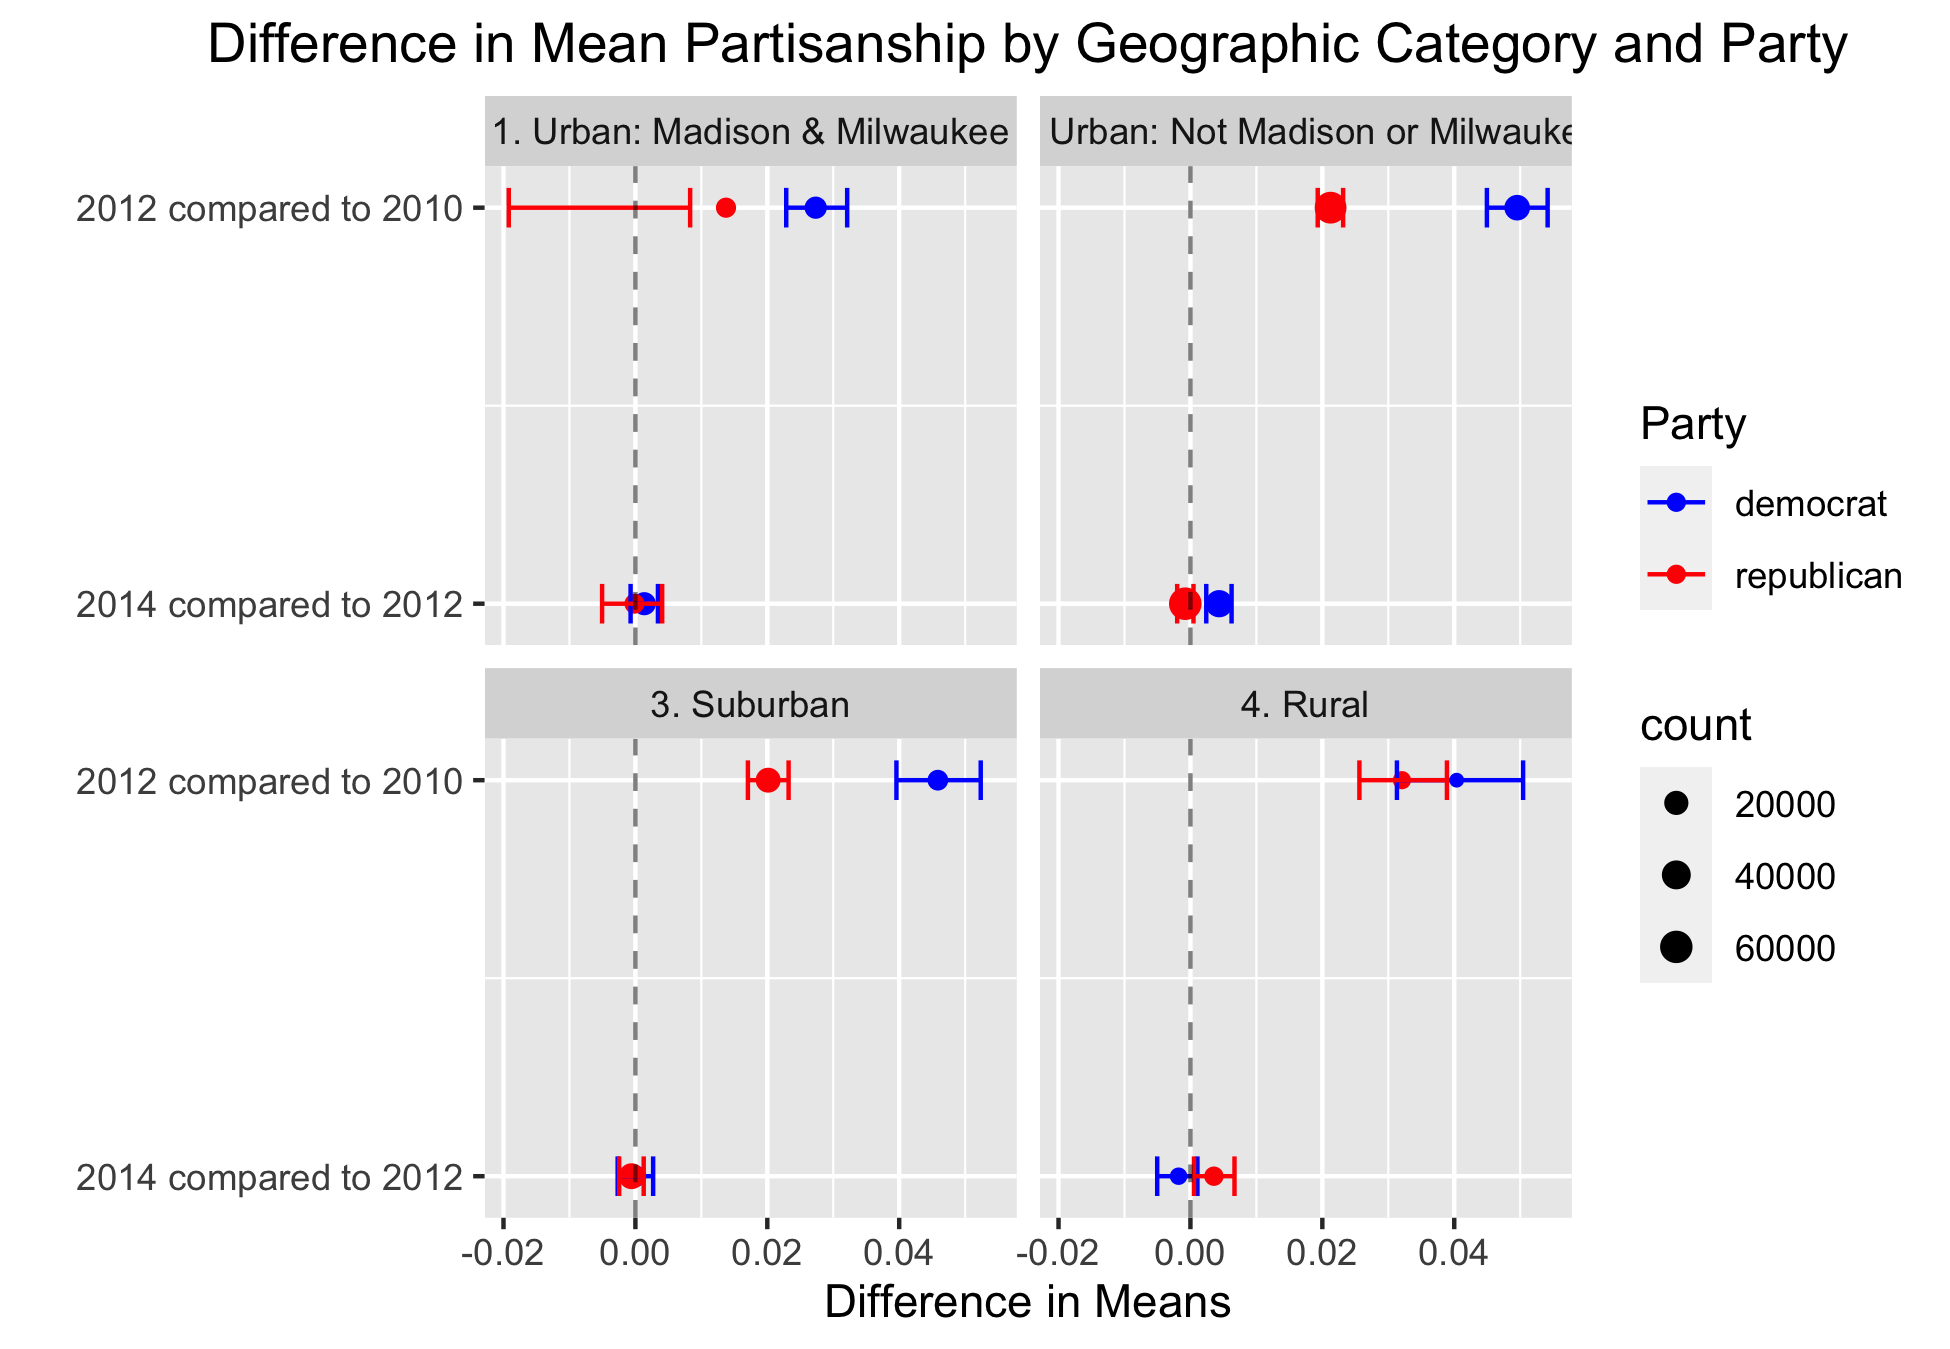
\includegraphics{geo_and_parties.png} To further analyze the partisan
trends between Democrats and Republicans, I ran the same bootstrapping
test for both parties in each of the geographic categories. In the 2012
compared to 2010 cycle, both parties had a significant mean difference
in partisanship across the entire state, with Democrats consistently
increasing their partisanship compared to Republicans. This aligns with
the massive push to replace Governor Walker in the 2012 recall
elections. Interestingly, despite the efforts among Democratic donors,
the outcome of the election was not in their favor.

We can then move to note that in the 2014 to 2012 cycle, the Urban
excluding Madison and Milwaukee and the Rural categories still had
significant differences in partisanship. With this in mind, running the
bootstrapping test allows us to see if this was true across both parties
in these regions. The results of the test show that this was not the
case. Somewhat unsurprisingly, only the Republican donors had a
significant difference in partisanship from 2012 to 2014. This can
possibly be linked to the growing ``rural consciousness'' that rural
Republicans felt as they continued to identify with Scott Walker's
ideas. On the other hand, in urban Wisconsin outside of the two major
cities, it was Democratic donors that had a super significant difference
in partisanship in 2014 while Republican donors remained
unchanged\ldots{}

\newpage

\hypertarget{extracting-key-cities-from-the-geographic-category-2.-urban.-not-madison-or-milwaukee}{%
\subsection{Extracting key cities from the geographic category `2.
Urban. Not Madison or
Milwaukee'}\label{extracting-key-cities-from-the-geographic-category-2.-urban.-not-madison-or-milwaukee}}

Data taken from \url{https://www.unitedstateszipcodes.org/wi/}

\newpage

\hypertarget{comparing-old-and-new-donors-for-a-given-election-year}{%
\subsection{Comparing Old and New Donors (for a given election
year)}\label{comparing-old-and-new-donors-for-a-given-election-year}}

\begin{longtable}[]{@{}lrll@{}}
\caption{Bootstrapped difference-in-means test with 1,000 replications
comparing mean partisanship of new versus old donors.}\tabularnewline
\toprule
Election Year & Diff. & CI & p\tabularnewline
\midrule
\endfirsthead
\toprule
Election Year & Diff. & CI & p\tabularnewline
\midrule
\endhead
2012 & 0.02277 & 0.02093-0.02477 & \textless.001\tabularnewline
2014 & 0.00708 & 0.00606-0.00809 & \textless.001\tabularnewline
\bottomrule
\end{longtable}

\newpage

\begin{verbatim}
## `summarise()` has grouped output by 'election_year', 'geo_category'. You can override using the `.groups` argument.
\end{verbatim}

\begin{verbatim}
## `summarise()` has grouped output by 'election_year'. You can override using the `.groups` argument.
\end{verbatim}

\begin{verbatim}
## Joining, by = c("election_year", "geo_category")
\end{verbatim}

\begin{verbatim}
## `summarise()` has grouped output by 'election_year', 'geo_category'. You can override using the `.groups` argument.
\end{verbatim}

\begin{verbatim}
## `summarise()` has grouped output by 'election_year'. You can override using the `.groups` argument.
\end{verbatim}

\begin{verbatim}
## Joining, by = c("election_year", "party_bin")
\end{verbatim}

\begin{verbatim}
## Joining, by = c("election_year", "geo_category")
\end{verbatim}

\begin{longtable}[]{@{}llrrrrrr@{}}
\caption{Number of Donors, Proportion of Donations, and Percentage of
Donors from each Geographic Category per Year}\tabularnewline
\toprule
\begin{minipage}[b]{0.07\columnwidth}\raggedright
Election Year\strut
\end{minipage} & \begin{minipage}[b]{0.17\columnwidth}\raggedright
Geographic Cateogory\strut
\end{minipage} & \begin{minipage}[b]{0.09\columnwidth}\raggedleft
Democratic Donors\strut
\end{minipage} & \begin{minipage}[b]{0.09\columnwidth}\raggedleft
Republican Donors\strut
\end{minipage} & \begin{minipage}[b]{0.08\columnwidth}\raggedleft
\% Dem donations\strut
\end{minipage} & \begin{minipage}[b]{0.08\columnwidth}\raggedleft
\% Rep donations\strut
\end{minipage} & \begin{minipage}[b]{0.11\columnwidth}\raggedleft
\% of yearly Dem donors\strut
\end{minipage} & \begin{minipage}[b]{0.11\columnwidth}\raggedleft
\% of yearly Rep donors\strut
\end{minipage}\tabularnewline
\midrule
\endfirsthead
\toprule
\begin{minipage}[b]{0.07\columnwidth}\raggedright
Election Year\strut
\end{minipage} & \begin{minipage}[b]{0.17\columnwidth}\raggedright
Geographic Cateogory\strut
\end{minipage} & \begin{minipage}[b]{0.09\columnwidth}\raggedleft
Democratic Donors\strut
\end{minipage} & \begin{minipage}[b]{0.09\columnwidth}\raggedleft
Republican Donors\strut
\end{minipage} & \begin{minipage}[b]{0.08\columnwidth}\raggedleft
\% Dem donations\strut
\end{minipage} & \begin{minipage}[b]{0.08\columnwidth}\raggedleft
\% Rep donations\strut
\end{minipage} & \begin{minipage}[b]{0.11\columnwidth}\raggedleft
\% of yearly Dem donors\strut
\end{minipage} & \begin{minipage}[b]{0.11\columnwidth}\raggedleft
\% of yearly Rep donors\strut
\end{minipage}\tabularnewline
\midrule
\endhead
\begin{minipage}[t]{0.07\columnwidth}\raggedright
2010\strut
\end{minipage} & \begin{minipage}[t]{0.17\columnwidth}\raggedright
1. Urban: Madison \& Milwaukee\strut
\end{minipage} & \begin{minipage}[t]{0.09\columnwidth}\raggedleft
4790\strut
\end{minipage} & \begin{minipage}[t]{0.09\columnwidth}\raggedleft
4118\strut
\end{minipage} & \begin{minipage}[t]{0.08\columnwidth}\raggedleft
0.5588885\strut
\end{minipage} & \begin{minipage}[t]{0.08\columnwidth}\raggedleft
0.4411115\strut
\end{minipage} & \begin{minipage}[t]{0.11\columnwidth}\raggedleft
0.2778583\strut
\end{minipage} & \begin{minipage}[t]{0.11\columnwidth}\raggedleft
0.1143254\strut
\end{minipage}\tabularnewline
\begin{minipage}[t]{0.07\columnwidth}\raggedright
2010\strut
\end{minipage} & \begin{minipage}[t]{0.17\columnwidth}\raggedright
2. Urban: Not Madison or Milwaukee\strut
\end{minipage} & \begin{minipage}[t]{0.09\columnwidth}\raggedleft
7839\strut
\end{minipage} & \begin{minipage}[t]{0.09\columnwidth}\raggedleft
21643\strut
\end{minipage} & \begin{minipage}[t]{0.08\columnwidth}\raggedleft
0.1782203\strut
\end{minipage} & \begin{minipage}[t]{0.08\columnwidth}\raggedleft
0.8217797\strut
\end{minipage} & \begin{minipage}[t]{0.11\columnwidth}\raggedleft
0.4547248\strut
\end{minipage} & \begin{minipage}[t]{0.11\columnwidth}\raggedleft
0.6008606\strut
\end{minipage}\tabularnewline
\begin{minipage}[t]{0.07\columnwidth}\raggedright
2010\strut
\end{minipage} & \begin{minipage}[t]{0.17\columnwidth}\raggedright
3. Suburban\strut
\end{minipage} & \begin{minipage}[t]{0.09\columnwidth}\raggedleft
3366\strut
\end{minipage} & \begin{minipage}[t]{0.09\columnwidth}\raggedleft
8288\strut
\end{minipage} & \begin{minipage}[t]{0.08\columnwidth}\raggedleft
0.2887292\strut
\end{minipage} & \begin{minipage}[t]{0.08\columnwidth}\raggedleft
0.7112708\strut
\end{minipage} & \begin{minipage}[t]{0.11\columnwidth}\raggedleft
0.1952549\strut
\end{minipage} & \begin{minipage}[t]{0.11\columnwidth}\raggedleft
0.2300944\strut
\end{minipage}\tabularnewline
\begin{minipage}[t]{0.07\columnwidth}\raggedright
2010\strut
\end{minipage} & \begin{minipage}[t]{0.17\columnwidth}\raggedright
4. Rural\strut
\end{minipage} & \begin{minipage}[t]{0.09\columnwidth}\raggedleft
1244\strut
\end{minipage} & \begin{minipage}[t]{0.09\columnwidth}\raggedleft
1971\strut
\end{minipage} & \begin{minipage}[t]{0.08\columnwidth}\raggedleft
0.3682188\strut
\end{minipage} & \begin{minipage}[t]{0.08\columnwidth}\raggedleft
0.6317812\strut
\end{minipage} & \begin{minipage}[t]{0.11\columnwidth}\raggedleft
0.0721620\strut
\end{minipage} & \begin{minipage}[t]{0.11\columnwidth}\raggedleft
0.0547196\strut
\end{minipage}\tabularnewline
\begin{minipage}[t]{0.07\columnwidth}\raggedright
2012\strut
\end{minipage} & \begin{minipage}[t]{0.17\columnwidth}\raggedright
1. Urban: Madison \& Milwaukee\strut
\end{minipage} & \begin{minipage}[t]{0.09\columnwidth}\raggedleft
9294\strut
\end{minipage} & \begin{minipage}[t]{0.09\columnwidth}\raggedleft
5282\strut
\end{minipage} & \begin{minipage}[t]{0.08\columnwidth}\raggedleft
0.4372746\strut
\end{minipage} & \begin{minipage}[t]{0.08\columnwidth}\raggedleft
0.5627254\strut
\end{minipage} & \begin{minipage}[t]{0.11\columnwidth}\raggedleft
0.2526917\strut
\end{minipage} & \begin{minipage}[t]{0.11\columnwidth}\raggedleft
0.0904777\strut
\end{minipage}\tabularnewline
\begin{minipage}[t]{0.07\columnwidth}\raggedright
2012\strut
\end{minipage} & \begin{minipage}[t]{0.17\columnwidth}\raggedright
2. Urban: Not Madison or Milwaukee\strut
\end{minipage} & \begin{minipage}[t]{0.09\columnwidth}\raggedleft
17291\strut
\end{minipage} & \begin{minipage}[t]{0.09\columnwidth}\raggedleft
34427\strut
\end{minipage} & \begin{minipage}[t]{0.08\columnwidth}\raggedleft
0.2616590\strut
\end{minipage} & \begin{minipage}[t]{0.08\columnwidth}\raggedleft
0.7383410\strut
\end{minipage} & \begin{minipage}[t]{0.11\columnwidth}\raggedleft
0.4701196\strut
\end{minipage} & \begin{minipage}[t]{0.11\columnwidth}\raggedleft
0.5897155\strut
\end{minipage}\tabularnewline
\begin{minipage}[t]{0.07\columnwidth}\raggedright
2012\strut
\end{minipage} & \begin{minipage}[t]{0.17\columnwidth}\raggedright
3. Suburban\strut
\end{minipage} & \begin{minipage}[t]{0.09\columnwidth}\raggedleft
7215\strut
\end{minipage} & \begin{minipage}[t]{0.09\columnwidth}\raggedleft
14317\strut
\end{minipage} & \begin{minipage}[t]{0.08\columnwidth}\raggedleft
0.2648979\strut
\end{minipage} & \begin{minipage}[t]{0.08\columnwidth}\raggedleft
0.7351021\strut
\end{minipage} & \begin{minipage}[t]{0.11\columnwidth}\raggedleft
0.1961664\strut
\end{minipage} & \begin{minipage}[t]{0.11\columnwidth}\raggedleft
0.2452423\strut
\end{minipage}\tabularnewline
\begin{minipage}[t]{0.07\columnwidth}\raggedright
2012\strut
\end{minipage} & \begin{minipage}[t]{0.17\columnwidth}\raggedright
4. Rural\strut
\end{minipage} & \begin{minipage}[t]{0.09\columnwidth}\raggedleft
2980\strut
\end{minipage} & \begin{minipage}[t]{0.09\columnwidth}\raggedleft
4353\strut
\end{minipage} & \begin{minipage}[t]{0.08\columnwidth}\raggedleft
0.3257401\strut
\end{minipage} & \begin{minipage}[t]{0.08\columnwidth}\raggedleft
0.6742599\strut
\end{minipage} & \begin{minipage}[t]{0.11\columnwidth}\raggedleft
0.0810223\strut
\end{minipage} & \begin{minipage}[t]{0.11\columnwidth}\raggedleft
0.0745645\strut
\end{minipage}\tabularnewline
\begin{minipage}[t]{0.07\columnwidth}\raggedright
2014\strut
\end{minipage} & \begin{minipage}[t]{0.17\columnwidth}\raggedright
1. Urban: Madison \& Milwaukee\strut
\end{minipage} & \begin{minipage}[t]{0.09\columnwidth}\raggedleft
7373\strut
\end{minipage} & \begin{minipage}[t]{0.09\columnwidth}\raggedleft
3758\strut
\end{minipage} & \begin{minipage}[t]{0.08\columnwidth}\raggedleft
0.6360548\strut
\end{minipage} & \begin{minipage}[t]{0.08\columnwidth}\raggedleft
0.3639452\strut
\end{minipage} & \begin{minipage}[t]{0.11\columnwidth}\raggedleft
0.2373869\strut
\end{minipage} & \begin{minipage}[t]{0.11\columnwidth}\raggedleft
0.0822032\strut
\end{minipage}\tabularnewline
\begin{minipage}[t]{0.07\columnwidth}\raggedright
2014\strut
\end{minipage} & \begin{minipage}[t]{0.17\columnwidth}\raggedright
2. Urban: Not Madison or Milwaukee\strut
\end{minipage} & \begin{minipage}[t]{0.09\columnwidth}\raggedleft
14623\strut
\end{minipage} & \begin{minipage}[t]{0.09\columnwidth}\raggedleft
26515\strut
\end{minipage} & \begin{minipage}[t]{0.08\columnwidth}\raggedleft
0.2661293\strut
\end{minipage} & \begin{minipage}[t]{0.08\columnwidth}\raggedleft
0.7338707\strut
\end{minipage} & \begin{minipage}[t]{0.11\columnwidth}\raggedleft
0.4708136\strut
\end{minipage} & \begin{minipage}[t]{0.11\columnwidth}\raggedleft
0.5799939\strut
\end{minipage}\tabularnewline
\begin{minipage}[t]{0.07\columnwidth}\raggedright
2014\strut
\end{minipage} & \begin{minipage}[t]{0.17\columnwidth}\raggedright
3. Suburban\strut
\end{minipage} & \begin{minipage}[t]{0.09\columnwidth}\raggedleft
6552\strut
\end{minipage} & \begin{minipage}[t]{0.09\columnwidth}\raggedleft
11796\strut
\end{minipage} & \begin{minipage}[t]{0.08\columnwidth}\raggedleft
0.2735117\strut
\end{minipage} & \begin{minipage}[t]{0.08\columnwidth}\raggedleft
0.7264883\strut
\end{minipage} & \begin{minipage}[t]{0.11\columnwidth}\raggedleft
0.2109533\strut
\end{minipage} & \begin{minipage}[t]{0.11\columnwidth}\raggedleft
0.2580278\strut
\end{minipage}\tabularnewline
\begin{minipage}[t]{0.07\columnwidth}\raggedright
2014\strut
\end{minipage} & \begin{minipage}[t]{0.17\columnwidth}\raggedright
4. Rural\strut
\end{minipage} & \begin{minipage}[t]{0.09\columnwidth}\raggedleft
2511\strut
\end{minipage} & \begin{minipage}[t]{0.09\columnwidth}\raggedleft
3647\strut
\end{minipage} & \begin{minipage}[t]{0.08\columnwidth}\raggedleft
0.3036583\strut
\end{minipage} & \begin{minipage}[t]{0.08\columnwidth}\raggedleft
0.6963417\strut
\end{minipage} & \begin{minipage}[t]{0.11\columnwidth}\raggedleft
0.0808461\strut
\end{minipage} & \begin{minipage}[t]{0.11\columnwidth}\raggedleft
0.0797751\strut
\end{minipage}\tabularnewline
\bottomrule
\end{longtable}

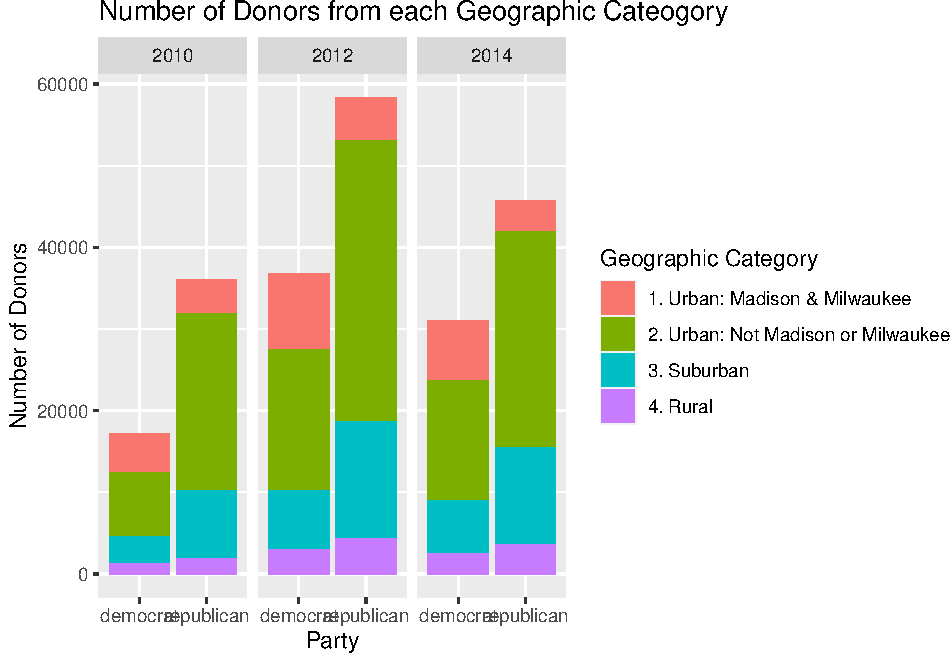
\includegraphics{scratch_files/figure-latex/unnamed-chunk-16-1.pdf}

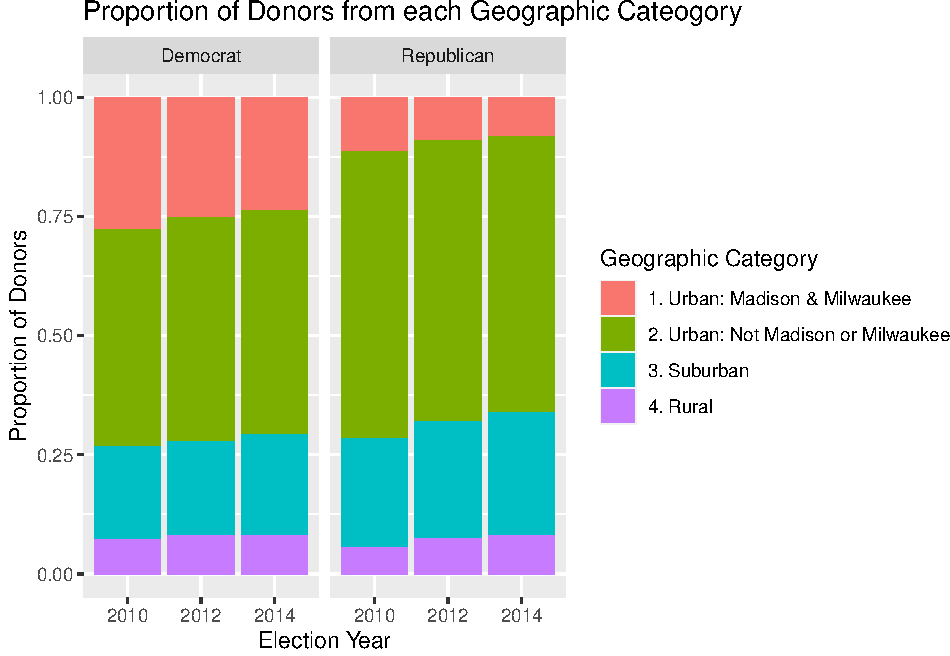
\includegraphics{scratch_files/figure-latex/unnamed-chunk-17-1.pdf}

The first plot shows the number of donors in each geographic category by
party and year, while the second graph breaks it down by percentages to
see where donors are coming from. It is obvious that the divisive
election of 2012 was reflected in a huge influx of donors from both
parties. Looking at the proportions, we see that the distribution of
donors across geographic categories remained largely consistent across
election years. Republican donors came from predominately the
non-Madison-or-Milwaukee urban category, while the Democratic party was
dominated by the two urban regions.

\newpage

\hypertarget{incorprating-size-of-donations}{%
\subsection{Incorprating Size of
Donations}\label{incorprating-size-of-donations}}

\hypertarget{use-200-cutoff-to-compare-small-and-large-donors}{%
\subsubsection{Use \$200 cutoff to compare small and large
donors}\label{use-200-cutoff-to-compare-small-and-large-donors}}

\begin{longtable}[]{@{}lrll@{}}
\caption{Bootstrapped difference-in-means test with 1,000 replications
comparing mean partisanship of small versus big donors.}\tabularnewline
\toprule
Election Year & Diff. & CI & p\tabularnewline
\midrule
\endfirsthead
\toprule
Election Year & Diff. & CI & p\tabularnewline
\midrule
\endhead
2010 & 0.05306 & 0.04897-0.05669 & \textless.001\tabularnewline
2012 & 0.01185 & 0.01084-0.01288 & \textless.001\tabularnewline
2014 & 0.01047 & 0.00936-0.01157 & \textless.001\tabularnewline
\bottomrule
\end{longtable}

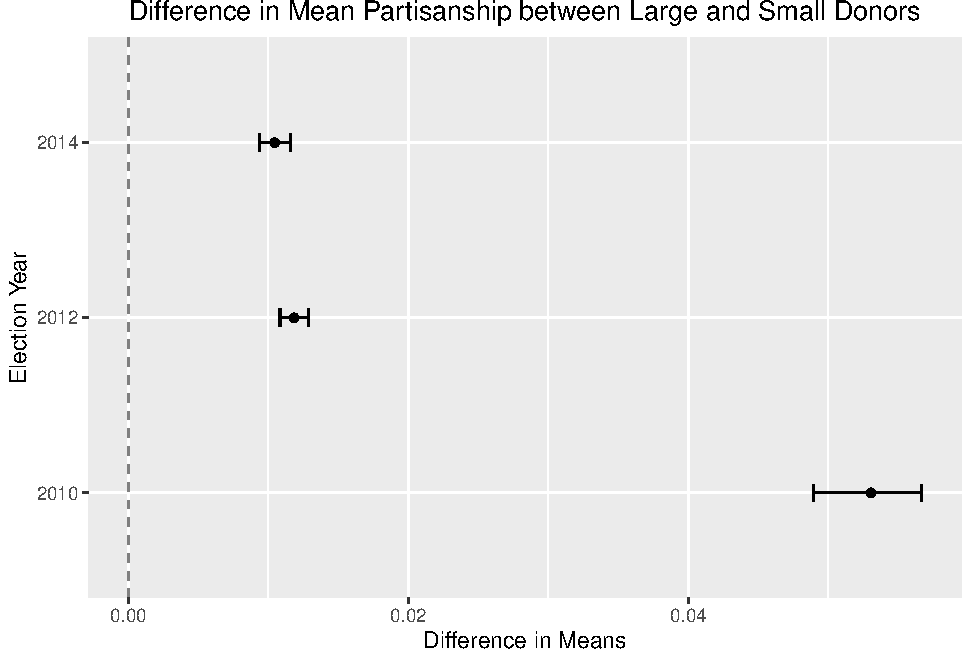
\includegraphics{scratch_files/figure-latex/unnamed-chunk-20-1.pdf}

From the results, small donors are significantly more polarized compared
to big donors in all election years.

\newpage

\hypertarget{different-urbanrural-classifications}{%
\subsection{Different Urban/Rural
Classifications}\label{different-urbanrural-classifications}}

\hypertarget{urban-inflence-codes-2013}{%
\subsubsection{Urban Inflence Codes
(2013)}\label{urban-inflence-codes-2013}}

From \url{https://www.ugpti.org/resources/reports/downloads/dp-207.pdf}

``The Economic Research Service uses metropolitan, micropolitan, and
non-core designations; population; and proximity to large urban areas to
classify counties using its Urban Influence Code system. Micropolitan
Statistical Areas are similar to Metropolitan Areas with the exception
that the core urban area must have at least 10,000 residents.
Metropolitan and Micropolitan Statistical Areas are jointly referred to
as Core Based Statistical Areas. The Urban Influence system is intended
to capture the role of urban areas and access on economic opportunity.''

Using Urban Influence Codes might be an attractive option because it
aims to classify geography by access to economic opportunity, which
links to the rural resentment felt by nonmetropolitan Wisconsinites.
Also the finer distinctions between nonmetro areas might be useful to
separate and look at.

\begin{longtable}[]{@{}ll@{}}
\caption{Urban Influence Codes}\tabularnewline
\toprule
\begin{minipage}[b]{0.16\columnwidth}\raggedright
Geographic Cateogry\strut
\end{minipage} & \begin{minipage}[b]{0.78\columnwidth}\raggedright
Description\strut
\end{minipage}\tabularnewline
\midrule
\endfirsthead
\toprule
\begin{minipage}[b]{0.16\columnwidth}\raggedright
Geographic Cateogry\strut
\end{minipage} & \begin{minipage}[b]{0.78\columnwidth}\raggedright
Description\strut
\end{minipage}\tabularnewline
\midrule
\endhead
\begin{minipage}[t]{0.16\columnwidth}\raggedright
1 Metropolitan\strut
\end{minipage} & \begin{minipage}[t]{0.78\columnwidth}\raggedright
In large metro area of 1+ million residents\strut
\end{minipage}\tabularnewline
\begin{minipage}[t]{0.16\columnwidth}\raggedright
2 Metropolitan\strut
\end{minipage} & \begin{minipage}[t]{0.78\columnwidth}\raggedright
In small metro area of less than 1 million residents\strut
\end{minipage}\tabularnewline
\begin{minipage}[t]{0.16\columnwidth}\raggedright
3 Nonmetropolitan\strut
\end{minipage} & \begin{minipage}[t]{0.78\columnwidth}\raggedright
Micropolitan area adjacent to large metro area\strut
\end{minipage}\tabularnewline
\begin{minipage}[t]{0.16\columnwidth}\raggedright
4 Nonmetropolitan\strut
\end{minipage} & \begin{minipage}[t]{0.78\columnwidth}\raggedright
Noncore adjacent to large metro area\strut
\end{minipage}\tabularnewline
\begin{minipage}[t]{0.16\columnwidth}\raggedright
5 Nonmetropolitan\strut
\end{minipage} & \begin{minipage}[t]{0.78\columnwidth}\raggedright
Micropolitan area adjacent to small metro area\strut
\end{minipage}\tabularnewline
\begin{minipage}[t]{0.16\columnwidth}\raggedright
6 Nonmetropolitan\strut
\end{minipage} & \begin{minipage}[t]{0.78\columnwidth}\raggedright
Noncore adjacent to small metro area and contains a town of at least
2,500 residents\strut
\end{minipage}\tabularnewline
\begin{minipage}[t]{0.16\columnwidth}\raggedright
7 Nonmetropolitan\strut
\end{minipage} & \begin{minipage}[t]{0.78\columnwidth}\raggedright
Noncore adjacent to small metro area and does not contain a town of at
least 2,500 residents\strut
\end{minipage}\tabularnewline
\begin{minipage}[t]{0.16\columnwidth}\raggedright
8 Nonmetropolitan\strut
\end{minipage} & \begin{minipage}[t]{0.78\columnwidth}\raggedright
Micropolitan area not adjacent to a metro area\strut
\end{minipage}\tabularnewline
\begin{minipage}[t]{0.16\columnwidth}\raggedright
9 Nonmetropolitan\strut
\end{minipage} & \begin{minipage}[t]{0.78\columnwidth}\raggedright
Noncore adjacent to micro area and contains a town of at least 2,500
residents\strut
\end{minipage}\tabularnewline
\begin{minipage}[t]{0.16\columnwidth}\raggedright
10 Nonmetropolitan\strut
\end{minipage} & \begin{minipage}[t]{0.78\columnwidth}\raggedright
Noncore adjacent to micro area and does not contain a town of at least
2,500 residents\strut
\end{minipage}\tabularnewline
\begin{minipage}[t]{0.16\columnwidth}\raggedright
11 Nonmetropolitan\strut
\end{minipage} & \begin{minipage}[t]{0.78\columnwidth}\raggedright
Noncore not adjacent to metro or micro area and contains a town of at
least 2,500 residents\strut
\end{minipage}\tabularnewline
\begin{minipage}[t]{0.16\columnwidth}\raggedright
12 Nonmetropolitan\strut
\end{minipage} & \begin{minipage}[t]{0.78\columnwidth}\raggedright
Noncore not adjacent to metro or micro area and does not contain a town
of at least 2,500 residents\strut
\end{minipage}\tabularnewline
\bottomrule
\end{longtable}

I decided to recode the donors by UIC codes similarly to the RUCC
categories: 2 urban, one suburban, and one rural category. I summarized
the donors in the table below.

\begin{verbatim}
## `summarise()` has grouped output by 'election_year', 'geo_category'. You can override using the `.groups` argument.
\end{verbatim}

\begin{verbatim}
## `summarise()` has grouped output by 'election_year'. You can override using the `.groups` argument.
\end{verbatim}

\begin{verbatim}
## Joining, by = c("election_year", "geo_category")
\end{verbatim}

\begin{verbatim}
## `summarise()` has grouped output by 'election_year', 'geo_category'. You can override using the `.groups` argument.
\end{verbatim}

\begin{verbatim}
## `summarise()` has grouped output by 'election_year'. You can override using the `.groups` argument.
\end{verbatim}

\begin{verbatim}
## Joining, by = c("election_year", "party_bin")
\end{verbatim}

\begin{verbatim}
## Joining, by = c("election_year", "geo_category")
\end{verbatim}

\begin{longtable}[]{@{}llrrrrrr@{}}
\caption{Number of Donors, Proportion of Donations, and Percentage of
Donors from each Geographic Category per Year}\tabularnewline
\toprule
\begin{minipage}[b]{0.07\columnwidth}\raggedright
Election Year\strut
\end{minipage} & \begin{minipage}[b]{0.19\columnwidth}\raggedright
Geographic Cateogry\strut
\end{minipage} & \begin{minipage}[b]{0.08\columnwidth}\raggedleft
Democratic Donors\strut
\end{minipage} & \begin{minipage}[b]{0.08\columnwidth}\raggedleft
Republican Donors\strut
\end{minipage} & \begin{minipage}[b]{0.07\columnwidth}\raggedleft
\% Dem donations\strut
\end{minipage} & \begin{minipage}[b]{0.07\columnwidth}\raggedleft
\% Rep donations\strut
\end{minipage} & \begin{minipage}[b]{0.11\columnwidth}\raggedleft
\% of yearly Dem donors\strut
\end{minipage} & \begin{minipage}[b]{0.11\columnwidth}\raggedleft
\% of yearly Rep donors\strut
\end{minipage}\tabularnewline
\midrule
\endfirsthead
\toprule
\begin{minipage}[b]{0.07\columnwidth}\raggedright
Election Year\strut
\end{minipage} & \begin{minipage}[b]{0.19\columnwidth}\raggedright
Geographic Cateogry\strut
\end{minipage} & \begin{minipage}[b]{0.08\columnwidth}\raggedleft
Democratic Donors\strut
\end{minipage} & \begin{minipage}[b]{0.08\columnwidth}\raggedleft
Republican Donors\strut
\end{minipage} & \begin{minipage}[b]{0.07\columnwidth}\raggedleft
\% Dem donations\strut
\end{minipage} & \begin{minipage}[b]{0.07\columnwidth}\raggedleft
\% Rep donations\strut
\end{minipage} & \begin{minipage}[b]{0.11\columnwidth}\raggedleft
\% of yearly Dem donors\strut
\end{minipage} & \begin{minipage}[b]{0.11\columnwidth}\raggedleft
\% of yearly Rep donors\strut
\end{minipage}\tabularnewline
\midrule
\endhead
\begin{minipage}[t]{0.07\columnwidth}\raggedright
2010\strut
\end{minipage} & \begin{minipage}[t]{0.19\columnwidth}\raggedright
1. Urban: 1+ million residents\strut
\end{minipage} & \begin{minipage}[t]{0.08\columnwidth}\raggedleft
4871\strut
\end{minipage} & \begin{minipage}[t]{0.08\columnwidth}\raggedleft
13792\strut
\end{minipage} & \begin{minipage}[t]{0.07\columnwidth}\raggedleft
0.1859478\strut
\end{minipage} & \begin{minipage}[t]{0.07\columnwidth}\raggedleft
0.8140522\strut
\end{minipage} & \begin{minipage}[t]{0.11\columnwidth}\raggedleft
0.2825570\strut
\end{minipage} & \begin{minipage}[t]{0.11\columnwidth}\raggedleft
0.3828984\strut
\end{minipage}\tabularnewline
\begin{minipage}[t]{0.07\columnwidth}\raggedright
2010\strut
\end{minipage} & \begin{minipage}[t]{0.19\columnwidth}\raggedright
2. Urban: Less than 1 million residents\strut
\end{minipage} & \begin{minipage}[t]{0.08\columnwidth}\raggedleft
7758\strut
\end{minipage} & \begin{minipage}[t]{0.08\columnwidth}\raggedleft
11969\strut
\end{minipage} & \begin{minipage}[t]{0.07\columnwidth}\raggedleft
0.4295204\strut
\end{minipage} & \begin{minipage}[t]{0.07\columnwidth}\raggedleft
0.5704796\strut
\end{minipage} & \begin{minipage}[t]{0.11\columnwidth}\raggedleft
0.4500261\strut
\end{minipage} & \begin{minipage}[t]{0.11\columnwidth}\raggedleft
0.3322876\strut
\end{minipage}\tabularnewline
\begin{minipage}[t]{0.07\columnwidth}\raggedright
2010\strut
\end{minipage} & \begin{minipage}[t]{0.19\columnwidth}\raggedright
3. Micropolitan\strut
\end{minipage} & \begin{minipage}[t]{0.08\columnwidth}\raggedleft
2230\strut
\end{minipage} & \begin{minipage}[t]{0.08\columnwidth}\raggedleft
5864\strut
\end{minipage} & \begin{minipage}[t]{0.07\columnwidth}\raggedleft
0.2794214\strut
\end{minipage} & \begin{minipage}[t]{0.07\columnwidth}\raggedleft
0.7205786\strut
\end{minipage} & \begin{minipage}[t]{0.11\columnwidth}\raggedleft
0.1293579\strut
\end{minipage} & \begin{minipage}[t]{0.11\columnwidth}\raggedleft
0.1627984\strut
\end{minipage}\tabularnewline
\begin{minipage}[t]{0.07\columnwidth}\raggedright
2010\strut
\end{minipage} & \begin{minipage}[t]{0.19\columnwidth}\raggedright
4. Noncore\strut
\end{minipage} & \begin{minipage}[t]{0.08\columnwidth}\raggedleft
2380\strut
\end{minipage} & \begin{minipage}[t]{0.08\columnwidth}\raggedleft
4395\strut
\end{minipage} & \begin{minipage}[t]{0.07\columnwidth}\raggedleft
0.3397248\strut
\end{minipage} & \begin{minipage}[t]{0.07\columnwidth}\raggedleft
0.6602752\strut
\end{minipage} & \begin{minipage}[t]{0.11\columnwidth}\raggedleft
0.1380591\strut
\end{minipage} & \begin{minipage}[t]{0.11\columnwidth}\raggedleft
0.1220155\strut
\end{minipage}\tabularnewline
\begin{minipage}[t]{0.07\columnwidth}\raggedright
2012\strut
\end{minipage} & \begin{minipage}[t]{0.19\columnwidth}\raggedright
1. Urban: 1+ million residents\strut
\end{minipage} & \begin{minipage}[t]{0.08\columnwidth}\raggedleft
8442\strut
\end{minipage} & \begin{minipage}[t]{0.08\columnwidth}\raggedleft
19592\strut
\end{minipage} & \begin{minipage}[t]{0.07\columnwidth}\raggedleft
0.2422605\strut
\end{minipage} & \begin{minipage}[t]{0.07\columnwidth}\raggedleft
0.7577395\strut
\end{minipage} & \begin{minipage}[t]{0.11\columnwidth}\raggedleft
0.2295269\strut
\end{minipage} & \begin{minipage}[t]{0.11\columnwidth}\raggedleft
0.3356001\strut
\end{minipage}\tabularnewline
\begin{minipage}[t]{0.07\columnwidth}\raggedright
2012\strut
\end{minipage} & \begin{minipage}[t]{0.19\columnwidth}\raggedright
2. Urban: Less than 1 million residents\strut
\end{minipage} & \begin{minipage}[t]{0.08\columnwidth}\raggedleft
18143\strut
\end{minipage} & \begin{minipage}[t]{0.08\columnwidth}\raggedleft
20117\strut
\end{minipage} & \begin{minipage}[t]{0.07\columnwidth}\raggedleft
0.3800353\strut
\end{minipage} & \begin{minipage}[t]{0.07\columnwidth}\raggedleft
0.6199647\strut
\end{minipage} & \begin{minipage}[t]{0.11\columnwidth}\raggedleft
0.4932844\strut
\end{minipage} & \begin{minipage}[t]{0.11\columnwidth}\raggedleft
0.3445931\strut
\end{minipage}\tabularnewline
\begin{minipage}[t]{0.07\columnwidth}\raggedright
2012\strut
\end{minipage} & \begin{minipage}[t]{0.19\columnwidth}\raggedright
3. Micropolitan\strut
\end{minipage} & \begin{minipage}[t]{0.08\columnwidth}\raggedleft
4813\strut
\end{minipage} & \begin{minipage}[t]{0.08\columnwidth}\raggedleft
9387\strut
\end{minipage} & \begin{minipage}[t]{0.07\columnwidth}\raggedleft
0.2628468\strut
\end{minipage} & \begin{minipage}[t]{0.07\columnwidth}\raggedleft
0.7371532\strut
\end{minipage} & \begin{minipage}[t]{0.11\columnwidth}\raggedleft
0.1308592\strut
\end{minipage} & \begin{minipage}[t]{0.11\columnwidth}\raggedleft
0.1607941\strut
\end{minipage}\tabularnewline
\begin{minipage}[t]{0.07\columnwidth}\raggedright
2012\strut
\end{minipage} & \begin{minipage}[t]{0.19\columnwidth}\raggedright
4. Noncore\strut
\end{minipage} & \begin{minipage}[t]{0.08\columnwidth}\raggedleft
5382\strut
\end{minipage} & \begin{minipage}[t]{0.08\columnwidth}\raggedleft
9283\strut
\end{minipage} & \begin{minipage}[t]{0.07\columnwidth}\raggedleft
0.2968777\strut
\end{minipage} & \begin{minipage}[t]{0.07\columnwidth}\raggedleft
0.7031223\strut
\end{minipage} & \begin{minipage}[t]{0.11\columnwidth}\raggedleft
0.1463295\strut
\end{minipage} & \begin{minipage}[t]{0.11\columnwidth}\raggedleft
0.1590127\strut
\end{minipage}\tabularnewline
\begin{minipage}[t]{0.07\columnwidth}\raggedright
2014\strut
\end{minipage} & \begin{minipage}[t]{0.19\columnwidth}\raggedright
1. Urban: 1+ million residents\strut
\end{minipage} & \begin{minipage}[t]{0.08\columnwidth}\raggedleft
6449\strut
\end{minipage} & \begin{minipage}[t]{0.08\columnwidth}\raggedleft
14214\strut
\end{minipage} & \begin{minipage}[t]{0.07\columnwidth}\raggedleft
0.2744927\strut
\end{minipage} & \begin{minipage}[t]{0.07\columnwidth}\raggedleft
0.7255073\strut
\end{minipage} & \begin{minipage}[t]{0.11\columnwidth}\raggedleft
0.2076371\strut
\end{minipage} & \begin{minipage}[t]{0.11\columnwidth}\raggedleft
0.3109196\strut
\end{minipage}\tabularnewline
\begin{minipage}[t]{0.07\columnwidth}\raggedright
2014\strut
\end{minipage} & \begin{minipage}[t]{0.19\columnwidth}\raggedright
2. Urban: Less than 1 million residents\strut
\end{minipage} & \begin{minipage}[t]{0.08\columnwidth}\raggedleft
15547\strut
\end{minipage} & \begin{minipage}[t]{0.08\columnwidth}\raggedleft
16059\strut
\end{minipage} & \begin{minipage}[t]{0.07\columnwidth}\raggedleft
0.4912612\strut
\end{minipage} & \begin{minipage}[t]{0.07\columnwidth}\raggedleft
0.5087388\strut
\end{minipage} & \begin{minipage}[t]{0.11\columnwidth}\raggedleft
0.5005634\strut
\end{minipage} & \begin{minipage}[t]{0.11\columnwidth}\raggedleft
0.3512775\strut
\end{minipage}\tabularnewline
\begin{minipage}[t]{0.07\columnwidth}\raggedright
2014\strut
\end{minipage} & \begin{minipage}[t]{0.19\columnwidth}\raggedright
3. Micropolitan\strut
\end{minipage} & \begin{minipage}[t]{0.08\columnwidth}\raggedleft
4023\strut
\end{minipage} & \begin{minipage}[t]{0.08\columnwidth}\raggedleft
7867\strut
\end{minipage} & \begin{minipage}[t]{0.07\columnwidth}\raggedleft
0.2453364\strut
\end{minipage} & \begin{minipage}[t]{0.07\columnwidth}\raggedleft
0.7546636\strut
\end{minipage} & \begin{minipage}[t]{0.11\columnwidth}\raggedleft
0.1295277\strut
\end{minipage} & \begin{minipage}[t]{0.11\columnwidth}\raggedleft
0.1720842\strut
\end{minipage}\tabularnewline
\begin{minipage}[t]{0.07\columnwidth}\raggedright
2014\strut
\end{minipage} & \begin{minipage}[t]{0.19\columnwidth}\raggedright
4. Noncore\strut
\end{minipage} & \begin{minipage}[t]{0.08\columnwidth}\raggedleft
5040\strut
\end{minipage} & \begin{minipage}[t]{0.08\columnwidth}\raggedleft
7576\strut
\end{minipage} & \begin{minipage}[t]{0.07\columnwidth}\raggedleft
0.3186539\strut
\end{minipage} & \begin{minipage}[t]{0.07\columnwidth}\raggedleft
0.6813461\strut
\end{minipage} & \begin{minipage}[t]{0.11\columnwidth}\raggedleft
0.1622718\strut
\end{minipage} & \begin{minipage}[t]{0.11\columnwidth}\raggedleft
0.1657188\strut
\end{minipage}\tabularnewline
\bottomrule
\end{longtable}

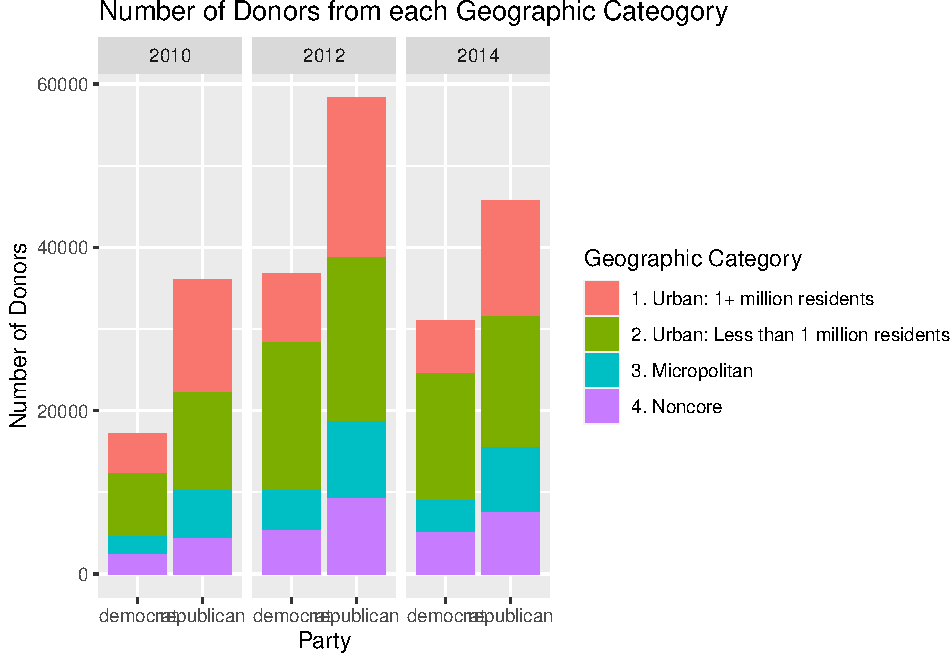
\includegraphics{scratch_files/figure-latex/unnamed-chunk-25-1.pdf}

The image looks very similar to the RUCC classification, except with
less suburban and more rural-classified donors. I ran the test on all
the categories without grouping.

\begin{longtable}[]{@{}llrll@{}}
\caption{Bootstrapped difference-in-means test with 1,000 replications
comparing mean partisanship by geographic category.}\tabularnewline
\toprule
Geographic Category & Election Year & Diff. & CI & p\tabularnewline
\midrule
\endfirsthead
\toprule
Geographic Category & Election Year & Diff. & CI & p\tabularnewline
\midrule
\endhead
1 & 2012 compared to 2010 & 0.02489 & 0.02233-0.02735 &
\textless.001\tabularnewline
2 & 2012 compared to 2010 & 0.04077 & 0.0379-0.04347 &
\textless.001\tabularnewline
3 & 2012 compared to 2010 & 0.02325 & 0.01899-0.02784 &
\textless.001\tabularnewline
4 & 2012 compared to 2010 & 0.02887 & 0.01716-0.04141 &
\textless.001\tabularnewline
5 & 2012 compared to 2010 & 0.04352 & 0.03635-0.05035 &
\textless.001\tabularnewline
6 & 2012 compared to 2010 & 0.04227 & 0.03647-0.04872 &
\textless.001\tabularnewline
7 & 2012 compared to 2010 & 0.03622 & 0.0201-0.05263 &
\textless.001\tabularnewline
8 & 2012 compared to 2010 & 0.04899 & -0.02675-0.15812 &
0.342\tabularnewline
9 & 2012 compared to 2010 & 0.06225 & 0.04641-0.07831 &
\textless.001\tabularnewline
11 & 2012 compared to 2010 & 0.01753 & 0.00388-0.03275 &
0.01\tabularnewline
12 & 2012 compared to 2010 & 0.04548 & 0.03105-0.06354 &
\textless.001\tabularnewline
1 & 2014 compared to 2012 & 0.00470 & 0.00313-0.00627 &
\textless.001\tabularnewline
2 & 2014 compared to 2012 & -0.00092 & -0.00241-0.00052 &
0.232\tabularnewline
3 & 2014 compared to 2012 & 0.00262 & 0.00013-0.00503 &
0.044\tabularnewline
4 & 2014 compared to 2012 & -0.00409 & -0.00954-0.00117 &
0.132\tabularnewline
5 & 2014 compared to 2012 & -0.00044 & -0.00453-0.00372 &
0.82\tabularnewline
6 & 2014 compared to 2012 & -0.00254 & -0.00541-0.00023 &
0.088\tabularnewline
7 & 2014 compared to 2012 & 0.00281 & -0.00707-0.01104 &
0.506\tabularnewline
8 & 2014 compared to 2012 & 0.01273 & -0.01362-0.04097 &
0.396\tabularnewline
9 & 2014 compared to 2012 & 0.00483 & -0.00059-0.00982 &
0.078\tabularnewline
11 & 2014 compared to 2012 & 0.00195 & -0.00609-0.01055 &
0.646\tabularnewline
12 & 2014 compared to 2012 & 0.00214 & -0.00183-0.00608 &
0.29\tabularnewline
\bottomrule
\end{longtable}

\begin{longtable}[]{@{}llrll@{}}
\caption{Bootstrapped difference-in-means test with 1,000 replications
comparing mean partisanship by geographic category.}\tabularnewline
\toprule
\begin{minipage}[b]{0.37\columnwidth}\raggedright
Geographic Category\strut
\end{minipage} & \begin{minipage}[b]{0.20\columnwidth}\raggedright
Election Year\strut
\end{minipage} & \begin{minipage}[b]{0.08\columnwidth}\raggedleft
Diff.\strut
\end{minipage} & \begin{minipage}[b]{0.16\columnwidth}\raggedright
CI\strut
\end{minipage} & \begin{minipage}[b]{0.05\columnwidth}\raggedright
p\strut
\end{minipage}\tabularnewline
\midrule
\endfirsthead
\toprule
\begin{minipage}[b]{0.37\columnwidth}\raggedright
Geographic Category\strut
\end{minipage} & \begin{minipage}[b]{0.20\columnwidth}\raggedright
Election Year\strut
\end{minipage} & \begin{minipage}[b]{0.08\columnwidth}\raggedleft
Diff.\strut
\end{minipage} & \begin{minipage}[b]{0.16\columnwidth}\raggedright
CI\strut
\end{minipage} & \begin{minipage}[b]{0.05\columnwidth}\raggedright
p\strut
\end{minipage}\tabularnewline
\midrule
\endhead
\begin{minipage}[t]{0.37\columnwidth}\raggedright
1. Urban: 1+ million residents\strut
\end{minipage} & \begin{minipage}[t]{0.20\columnwidth}\raggedright
2012 compared to 2010\strut
\end{minipage} & \begin{minipage}[t]{0.08\columnwidth}\raggedleft
0.02489\strut
\end{minipage} & \begin{minipage}[t]{0.16\columnwidth}\raggedright
0.02233-0.02735\strut
\end{minipage} & \begin{minipage}[t]{0.05\columnwidth}\raggedright
\textless.001\strut
\end{minipage}\tabularnewline
\begin{minipage}[t]{0.37\columnwidth}\raggedright
2. Urban: Less than 1 million residents\strut
\end{minipage} & \begin{minipage}[t]{0.20\columnwidth}\raggedright
2012 compared to 2010\strut
\end{minipage} & \begin{minipage}[t]{0.08\columnwidth}\raggedleft
0.04077\strut
\end{minipage} & \begin{minipage}[t]{0.16\columnwidth}\raggedright
0.0379-0.04347\strut
\end{minipage} & \begin{minipage}[t]{0.05\columnwidth}\raggedright
\textless.001\strut
\end{minipage}\tabularnewline
\begin{minipage}[t]{0.37\columnwidth}\raggedright
3. Micropolitan\strut
\end{minipage} & \begin{minipage}[t]{0.20\columnwidth}\raggedright
2012 compared to 2010\strut
\end{minipage} & \begin{minipage}[t]{0.08\columnwidth}\raggedleft
0.03169\strut
\end{minipage} & \begin{minipage}[t]{0.16\columnwidth}\raggedright
0.0277-0.0356\strut
\end{minipage} & \begin{minipage}[t]{0.05\columnwidth}\raggedright
\textless.001\strut
\end{minipage}\tabularnewline
\begin{minipage}[t]{0.37\columnwidth}\raggedright
4. Noncore\strut
\end{minipage} & \begin{minipage}[t]{0.20\columnwidth}\raggedright
2012 compared to 2010\strut
\end{minipage} & \begin{minipage}[t]{0.08\columnwidth}\raggedleft
0.04221\strut
\end{minipage} & \begin{minipage}[t]{0.16\columnwidth}\raggedright
0.03717-0.04699\strut
\end{minipage} & \begin{minipage}[t]{0.05\columnwidth}\raggedright
\textless.001\strut
\end{minipage}\tabularnewline
\begin{minipage}[t]{0.37\columnwidth}\raggedright
1. Urban: 1+ million residents\strut
\end{minipage} & \begin{minipage}[t]{0.20\columnwidth}\raggedright
2014 compared to 2012\strut
\end{minipage} & \begin{minipage}[t]{0.08\columnwidth}\raggedleft
0.00470\strut
\end{minipage} & \begin{minipage}[t]{0.16\columnwidth}\raggedright
0.00313-0.00627\strut
\end{minipage} & \begin{minipage}[t]{0.05\columnwidth}\raggedright
\textless.001\strut
\end{minipage}\tabularnewline
\begin{minipage}[t]{0.37\columnwidth}\raggedright
2. Urban: Less than 1 million residents\strut
\end{minipage} & \begin{minipage}[t]{0.20\columnwidth}\raggedright
2014 compared to 2012\strut
\end{minipage} & \begin{minipage}[t]{0.08\columnwidth}\raggedleft
-0.00092\strut
\end{minipage} & \begin{minipage}[t]{0.16\columnwidth}\raggedright
-0.00241-0.00052\strut
\end{minipage} & \begin{minipage}[t]{0.05\columnwidth}\raggedright
0.232\strut
\end{minipage}\tabularnewline
\begin{minipage}[t]{0.37\columnwidth}\raggedright
3. Micropolitan\strut
\end{minipage} & \begin{minipage}[t]{0.20\columnwidth}\raggedright
2014 compared to 2012\strut
\end{minipage} & \begin{minipage}[t]{0.08\columnwidth}\raggedleft
0.00104\strut
\end{minipage} & \begin{minipage}[t]{0.16\columnwidth}\raggedright
-0.00116-0.00322\strut
\end{minipage} & \begin{minipage}[t]{0.05\columnwidth}\raggedright
0.354\strut
\end{minipage}\tabularnewline
\begin{minipage}[t]{0.37\columnwidth}\raggedright
4. Noncore\strut
\end{minipage} & \begin{minipage}[t]{0.20\columnwidth}\raggedright
2014 compared to 2012\strut
\end{minipage} & \begin{minipage}[t]{0.08\columnwidth}\raggedleft
-0.00089\strut
\end{minipage} & \begin{minipage}[t]{0.16\columnwidth}\raggedright
-0.00294-0.0011\strut
\end{minipage} & \begin{minipage}[t]{0.05\columnwidth}\raggedright
0.42\strut
\end{minipage}\tabularnewline
\bottomrule
\end{longtable}

The difference-in-means test resulted in only the first urban category
to be significant, which is different from what the RUCC data gave us
(with both the 2nd urban category and rural significant). Finally, I
decided to group into six categories based on adjacency to urban areas
and ran the same test. Again, only the first category was significant
for the 2014 election cycle.

\begin{longtable}[]{@{}llrll@{}}
\caption{Bootstrapped difference-in-means test with 1,000 replications
comparing mean partisanship by geographic category.}\tabularnewline
\toprule
\begin{minipage}[b]{0.40\columnwidth}\raggedright
Geographic Category\strut
\end{minipage} & \begin{minipage}[b]{0.19\columnwidth}\raggedright
Election Year\strut
\end{minipage} & \begin{minipage}[b]{0.08\columnwidth}\raggedleft
Diff.\strut
\end{minipage} & \begin{minipage}[b]{0.14\columnwidth}\raggedright
CI\strut
\end{minipage} & \begin{minipage}[b]{0.05\columnwidth}\raggedright
p\strut
\end{minipage}\tabularnewline
\midrule
\endfirsthead
\toprule
\begin{minipage}[b]{0.40\columnwidth}\raggedright
Geographic Category\strut
\end{minipage} & \begin{minipage}[b]{0.19\columnwidth}\raggedright
Election Year\strut
\end{minipage} & \begin{minipage}[b]{0.08\columnwidth}\raggedleft
Diff.\strut
\end{minipage} & \begin{minipage}[b]{0.14\columnwidth}\raggedright
CI\strut
\end{minipage} & \begin{minipage}[b]{0.05\columnwidth}\raggedright
p\strut
\end{minipage}\tabularnewline
\midrule
\endhead
\begin{minipage}[t]{0.40\columnwidth}\raggedright
1. Urban: 1+ million residents\strut
\end{minipage} & \begin{minipage}[t]{0.19\columnwidth}\raggedright
2012 compared to 2010\strut
\end{minipage} & \begin{minipage}[t]{0.08\columnwidth}\raggedleft
0.02489\strut
\end{minipage} & \begin{minipage}[t]{0.14\columnwidth}\raggedright
0.02233-0.02735\strut
\end{minipage} & \begin{minipage}[t]{0.05\columnwidth}\raggedright
\textless.001\strut
\end{minipage}\tabularnewline
\begin{minipage}[t]{0.40\columnwidth}\raggedright
2. Urban: Less than 1 million residents\strut
\end{minipage} & \begin{minipage}[t]{0.19\columnwidth}\raggedright
2012 compared to 2010\strut
\end{minipage} & \begin{minipage}[t]{0.08\columnwidth}\raggedleft
0.04077\strut
\end{minipage} & \begin{minipage}[t]{0.14\columnwidth}\raggedright
0.0379-0.04347\strut
\end{minipage} & \begin{minipage}[t]{0.05\columnwidth}\raggedright
\textless.001\strut
\end{minipage}\tabularnewline
\begin{minipage}[t]{0.40\columnwidth}\raggedright
3. Micropolitan: Adjacent to an urban area\strut
\end{minipage} & \begin{minipage}[t]{0.19\columnwidth}\raggedright
2012 compared to 2010\strut
\end{minipage} & \begin{minipage}[t]{0.08\columnwidth}\raggedleft
0.03173\strut
\end{minipage} & \begin{minipage}[t]{0.14\columnwidth}\raggedright
0.02785-0.03589\strut
\end{minipage} & \begin{minipage}[t]{0.05\columnwidth}\raggedright
\textless.001\strut
\end{minipage}\tabularnewline
\begin{minipage}[t]{0.40\columnwidth}\raggedright
4. Micropolitan: Not adjacent to an urban area\strut
\end{minipage} & \begin{minipage}[t]{0.19\columnwidth}\raggedright
2012 compared to 2010\strut
\end{minipage} & \begin{minipage}[t]{0.08\columnwidth}\raggedleft
0.04575\strut
\end{minipage} & \begin{minipage}[t]{0.14\columnwidth}\raggedright
-0.03129-0.1419\strut
\end{minipage} & \begin{minipage}[t]{0.05\columnwidth}\raggedright
0.318\strut
\end{minipage}\tabularnewline
\begin{minipage}[t]{0.40\columnwidth}\raggedright
5. Noncore: Adjacent to a metro area\strut
\end{minipage} & \begin{minipage}[t]{0.19\columnwidth}\raggedright
2012 compared to 2010\strut
\end{minipage} & \begin{minipage}[t]{0.08\columnwidth}\raggedleft
0.04303\strut
\end{minipage} & \begin{minipage}[t]{0.14\columnwidth}\raggedright
0.03788-0.04805\strut
\end{minipage} & \begin{minipage}[t]{0.05\columnwidth}\raggedright
\textless.001\strut
\end{minipage}\tabularnewline
\begin{minipage}[t]{0.40\columnwidth}\raggedright
6. Noncore: Not Adjacent a metro area\strut
\end{minipage} & \begin{minipage}[t]{0.19\columnwidth}\raggedright
2012 compared to 2010\strut
\end{minipage} & \begin{minipage}[t]{0.08\columnwidth}\raggedleft
0.03552\strut
\end{minipage} & \begin{minipage}[t]{0.14\columnwidth}\raggedright
0.02443-0.0473\strut
\end{minipage} & \begin{minipage}[t]{0.05\columnwidth}\raggedright
\textless.001\strut
\end{minipage}\tabularnewline
\begin{minipage}[t]{0.40\columnwidth}\raggedright
1. Urban: 1+ million residents\strut
\end{minipage} & \begin{minipage}[t]{0.19\columnwidth}\raggedright
2014 compared to 2012\strut
\end{minipage} & \begin{minipage}[t]{0.08\columnwidth}\raggedleft
0.00470\strut
\end{minipage} & \begin{minipage}[t]{0.14\columnwidth}\raggedright
0.00313-0.00627\strut
\end{minipage} & \begin{minipage}[t]{0.05\columnwidth}\raggedright
\textless.001\strut
\end{minipage}\tabularnewline
\begin{minipage}[t]{0.40\columnwidth}\raggedright
2. Urban: Less than 1 million residents\strut
\end{minipage} & \begin{minipage}[t]{0.19\columnwidth}\raggedright
2014 compared to 2012\strut
\end{minipage} & \begin{minipage}[t]{0.08\columnwidth}\raggedleft
-0.00092\strut
\end{minipage} & \begin{minipage}[t]{0.14\columnwidth}\raggedright
-0.00241-0.00052\strut
\end{minipage} & \begin{minipage}[t]{0.05\columnwidth}\raggedright
0.232\strut
\end{minipage}\tabularnewline
\begin{minipage}[t]{0.40\columnwidth}\raggedright
3. Micropolitan: Adjacent to an urban area\strut
\end{minipage} & \begin{minipage}[t]{0.19\columnwidth}\raggedright
2014 compared to 2012\strut
\end{minipage} & \begin{minipage}[t]{0.08\columnwidth}\raggedleft
0.00097\strut
\end{minipage} & \begin{minipage}[t]{0.14\columnwidth}\raggedright
-0.00127-0.00313\strut
\end{minipage} & \begin{minipage}[t]{0.05\columnwidth}\raggedright
0.406\strut
\end{minipage}\tabularnewline
\begin{minipage}[t]{0.40\columnwidth}\raggedright
4. Micropolitan: Not adjacent to an urban area\strut
\end{minipage} & \begin{minipage}[t]{0.19\columnwidth}\raggedright
2014 compared to 2012\strut
\end{minipage} & \begin{minipage}[t]{0.08\columnwidth}\raggedleft
0.01311\strut
\end{minipage} & \begin{minipage}[t]{0.14\columnwidth}\raggedright
-0.01696-0.04348\strut
\end{minipage} & \begin{minipage}[t]{0.05\columnwidth}\raggedright
0.386\strut
\end{minipage}\tabularnewline
\begin{minipage}[t]{0.40\columnwidth}\raggedright
5. Noncore: Adjacent to a metro area\strut
\end{minipage} & \begin{minipage}[t]{0.19\columnwidth}\raggedright
2014 compared to 2012\strut
\end{minipage} & \begin{minipage}[t]{0.08\columnwidth}\raggedleft
-0.00133\strut
\end{minipage} & \begin{minipage}[t]{0.14\columnwidth}\raggedright
-0.00373-0.001\strut
\end{minipage} & \begin{minipage}[t]{0.05\columnwidth}\raggedright
0.286\strut
\end{minipage}\tabularnewline
\begin{minipage}[t]{0.40\columnwidth}\raggedright
6. Noncore: Not Adjacent a metro area\strut
\end{minipage} & \begin{minipage}[t]{0.19\columnwidth}\raggedright
2014 compared to 2012\strut
\end{minipage} & \begin{minipage}[t]{0.08\columnwidth}\raggedleft
0.00152\strut
\end{minipage} & \begin{minipage}[t]{0.14\columnwidth}\raggedright
-0.0023-0.00537\strut
\end{minipage} & \begin{minipage}[t]{0.05\columnwidth}\raggedright
0.466\strut
\end{minipage}\tabularnewline
\bottomrule
\end{longtable}

\newpage

\hypertarget{cdcs-2013-nchs-urbanrural-classification-scheme-for-counties}{%
\subsubsection{CDC's 2013 NCHS Urban--Rural Classification Scheme for
Counties}\label{cdcs-2013-nchs-urbanrural-classification-scheme-for-counties}}

From \url{https://www.cdc.gov/nchs/data/series/sr_02/sr02_166.pdf}

``A key feature of the NCHS urban-rural scheme, which makes it
particularly well-suited for health analyses, is that it separates
counties within large metropolitan areas (1 million or more population)
into two categories: large ``central'' metro (akin to inner cities) and
large ``fringe'' metro (akin to suburbs). This is an important feature
of the NCHS urban-rural scheme because for a number of health measures,
residents of large fringe metro areas fare substantially better than
residents of other urbanization levels. For these measures, residents of
the inner cities and suburbs of large metropolitan areas must be
differentiated to obtain an accurate characterization of health
disparities across the full urban-rural spectrum."

The NCHS classification scheme primarily uses population as its measure
of urbanization, and it tries to capture health (quality of life?) is
that urban areas are broken up more, with even more specificity between
a ``large central metro'' and a ``large fringe metro.'' I thought that
this turned out useful later. Also I didn't think regrouping was
necessary since the six categories seemed pretty clear.

\begin{longtable}[]{@{}ll@{}}
\caption{NCHS Urban-Rural Scheme}\tabularnewline
\toprule
\begin{minipage}[b]{0.07\columnwidth}\raggedright
Urbanization Level\strut
\end{minipage} & \begin{minipage}[b]{0.87\columnwidth}\raggedright
Classification Rules\strut
\end{minipage}\tabularnewline
\midrule
\endfirsthead
\toprule
\begin{minipage}[b]{0.07\columnwidth}\raggedright
Urbanization Level\strut
\end{minipage} & \begin{minipage}[b]{0.87\columnwidth}\raggedright
Classification Rules\strut
\end{minipage}\tabularnewline
\midrule
\endhead
\begin{minipage}[t]{0.07\columnwidth}\raggedright
1. Large Central Metro\strut
\end{minipage} & \begin{minipage}[t]{0.87\columnwidth}\raggedright
Counties in MSAs of 1 million or more population that: 1) Contain the
entire population of the largest principal city of the MSA, or 2) Have
their entire population contained in the largest principal city of the
MSA, or 3) Contain at least 250,000 inhabitants of any principal city of
the MSA\strut
\end{minipage}\tabularnewline
\begin{minipage}[t]{0.07\columnwidth}\raggedright
2. Large Fringe Metro\strut
\end{minipage} & \begin{minipage}[t]{0.87\columnwidth}\raggedright
Counties in MSAs of 1 million or more population that did not qualify as
large central metro counties\strut
\end{minipage}\tabularnewline
\begin{minipage}[t]{0.07\columnwidth}\raggedright
3. Medium Metro\strut
\end{minipage} & \begin{minipage}[t]{0.87\columnwidth}\raggedright
Counties in MSAs of populations of 250,000--999,999\strut
\end{minipage}\tabularnewline
\begin{minipage}[t]{0.07\columnwidth}\raggedright
4. Small Metro\strut
\end{minipage} & \begin{minipage}[t]{0.87\columnwidth}\raggedright
Counties in MSAs of populations less than 250,000\strut
\end{minipage}\tabularnewline
\begin{minipage}[t]{0.07\columnwidth}\raggedright
5. Micropolitan\strut
\end{minipage} & \begin{minipage}[t]{0.87\columnwidth}\raggedright
Counties in micropolitan statistical areas\strut
\end{minipage}\tabularnewline
\begin{minipage}[t]{0.07\columnwidth}\raggedright
6. Noncore\strut
\end{minipage} & \begin{minipage}[t]{0.87\columnwidth}\raggedright
Nonmetropolitan counties that did not qualify as micropolitan\strut
\end{minipage}\tabularnewline
\bottomrule
\end{longtable}

\begin{verbatim}
## `summarise()` has grouped output by 'election_year', 'geo_category'. You can override using the `.groups` argument.
\end{verbatim}

\begin{verbatim}
## `summarise()` has grouped output by 'election_year'. You can override using the `.groups` argument.
\end{verbatim}

\begin{verbatim}
## Joining, by = c("election_year", "geo_category")
\end{verbatim}

\begin{verbatim}
## `summarise()` has grouped output by 'election_year', 'geo_category'. You can override using the `.groups` argument.
\end{verbatim}

\begin{verbatim}
## `summarise()` has grouped output by 'election_year'. You can override using the `.groups` argument.
\end{verbatim}

\begin{verbatim}
## Joining, by = c("election_year", "party_bin")
\end{verbatim}

\begin{verbatim}
## Joining, by = c("election_year", "geo_category")
\end{verbatim}

\begin{longtable}[]{@{}llrrrrrr@{}}
\caption{Number of Donors, Proportion of Donations, and Percentage of
Donors from each Geographic Category per Year}\tabularnewline
\toprule
\begin{minipage}[b]{0.07\columnwidth}\raggedright
Election Year\strut
\end{minipage} & \begin{minipage}[b]{0.12\columnwidth}\raggedright
Geographic Cateogry\strut
\end{minipage} & \begin{minipage}[b]{0.09\columnwidth}\raggedleft
Democratic Donors\strut
\end{minipage} & \begin{minipage}[b]{0.09\columnwidth}\raggedleft
Republican Donors\strut
\end{minipage} & \begin{minipage}[b]{0.08\columnwidth}\raggedleft
\% Dem donations\strut
\end{minipage} & \begin{minipage}[b]{0.08\columnwidth}\raggedleft
\% Rep donations\strut
\end{minipage} & \begin{minipage}[b]{0.12\columnwidth}\raggedleft
\% of yearly Dem donors\strut
\end{minipage} & \begin{minipage}[b]{0.12\columnwidth}\raggedleft
\% of yearly Rep donors\strut
\end{minipage}\tabularnewline
\midrule
\endfirsthead
\toprule
\begin{minipage}[b]{0.07\columnwidth}\raggedright
Election Year\strut
\end{minipage} & \begin{minipage}[b]{0.12\columnwidth}\raggedright
Geographic Cateogry\strut
\end{minipage} & \begin{minipage}[b]{0.09\columnwidth}\raggedleft
Democratic Donors\strut
\end{minipage} & \begin{minipage}[b]{0.09\columnwidth}\raggedleft
Republican Donors\strut
\end{minipage} & \begin{minipage}[b]{0.08\columnwidth}\raggedleft
\% Dem donations\strut
\end{minipage} & \begin{minipage}[b]{0.08\columnwidth}\raggedleft
\% Rep donations\strut
\end{minipage} & \begin{minipage}[b]{0.12\columnwidth}\raggedleft
\% of yearly Dem donors\strut
\end{minipage} & \begin{minipage}[b]{0.12\columnwidth}\raggedleft
\% of yearly Rep donors\strut
\end{minipage}\tabularnewline
\midrule
\endhead
\begin{minipage}[t]{0.07\columnwidth}\raggedright
2010\strut
\end{minipage} & \begin{minipage}[t]{0.12\columnwidth}\raggedright
1. Large Central Metro\strut
\end{minipage} & \begin{minipage}[t]{0.09\columnwidth}\raggedleft
2796\strut
\end{minipage} & \begin{minipage}[t]{0.09\columnwidth}\raggedleft
4022\strut
\end{minipage} & \begin{minipage}[t]{0.08\columnwidth}\raggedleft
0.5115446\strut
\end{minipage} & \begin{minipage}[t]{0.08\columnwidth}\raggedleft
0.4884554\strut
\end{minipage} & \begin{minipage}[t]{0.12\columnwidth}\raggedleft
0.1621904\strut
\end{minipage} & \begin{minipage}[t]{0.12\columnwidth}\raggedleft
0.1116602\strut
\end{minipage}\tabularnewline
\begin{minipage}[t]{0.07\columnwidth}\raggedright
2010\strut
\end{minipage} & \begin{minipage}[t]{0.12\columnwidth}\raggedright
2. Large Fringe Metro\strut
\end{minipage} & \begin{minipage}[t]{0.09\columnwidth}\raggedleft
2075\strut
\end{minipage} & \begin{minipage}[t]{0.09\columnwidth}\raggedleft
9770\strut
\end{minipage} & \begin{minipage}[t]{0.08\columnwidth}\raggedleft
0.1034020\strut
\end{minipage} & \begin{minipage}[t]{0.08\columnwidth}\raggedleft
0.8965980\strut
\end{minipage} & \begin{minipage}[t]{0.12\columnwidth}\raggedleft
0.1203666\strut
\end{minipage} & \begin{minipage}[t]{0.12\columnwidth}\raggedleft
0.2712382\strut
\end{minipage}\tabularnewline
\begin{minipage}[t]{0.07\columnwidth}\raggedright
2010\strut
\end{minipage} & \begin{minipage}[t]{0.12\columnwidth}\raggedright
3. Medium Metro\strut
\end{minipage} & \begin{minipage}[t]{0.09\columnwidth}\raggedleft
3976\strut
\end{minipage} & \begin{minipage}[t]{0.09\columnwidth}\raggedleft
3659\strut
\end{minipage} & \begin{minipage}[t]{0.08\columnwidth}\raggedleft
0.5225614\strut
\end{minipage} & \begin{minipage}[t]{0.08\columnwidth}\raggedleft
0.4774386\strut
\end{minipage} & \begin{minipage}[t]{0.12\columnwidth}\raggedleft
0.2306398\strut
\end{minipage} & \begin{minipage}[t]{0.12\columnwidth}\raggedleft
0.1015825\strut
\end{minipage}\tabularnewline
\begin{minipage}[t]{0.07\columnwidth}\raggedright
2010\strut
\end{minipage} & \begin{minipage}[t]{0.12\columnwidth}\raggedright
4. Small Metro\strut
\end{minipage} & \begin{minipage}[t]{0.09\columnwidth}\raggedleft
3782\strut
\end{minipage} & \begin{minipage}[t]{0.09\columnwidth}\raggedleft
8310\strut
\end{minipage} & \begin{minipage}[t]{0.08\columnwidth}\raggedleft
0.3240419\strut
\end{minipage} & \begin{minipage}[t]{0.08\columnwidth}\raggedleft
0.6759581\strut
\end{minipage} & \begin{minipage}[t]{0.12\columnwidth}\raggedleft
0.2193863\strut
\end{minipage} & \begin{minipage}[t]{0.12\columnwidth}\raggedleft
0.2307052\strut
\end{minipage}\tabularnewline
\begin{minipage}[t]{0.07\columnwidth}\raggedright
2010\strut
\end{minipage} & \begin{minipage}[t]{0.12\columnwidth}\raggedright
5. Micropolitan\strut
\end{minipage} & \begin{minipage}[t]{0.09\columnwidth}\raggedleft
2230\strut
\end{minipage} & \begin{minipage}[t]{0.09\columnwidth}\raggedleft
5864\strut
\end{minipage} & \begin{minipage}[t]{0.08\columnwidth}\raggedleft
0.2794214\strut
\end{minipage} & \begin{minipage}[t]{0.08\columnwidth}\raggedleft
0.7205786\strut
\end{minipage} & \begin{minipage}[t]{0.12\columnwidth}\raggedleft
0.1293579\strut
\end{minipage} & \begin{minipage}[t]{0.12\columnwidth}\raggedleft
0.1627984\strut
\end{minipage}\tabularnewline
\begin{minipage}[t]{0.07\columnwidth}\raggedright
2010\strut
\end{minipage} & \begin{minipage}[t]{0.12\columnwidth}\raggedright
6. Noncore\strut
\end{minipage} & \begin{minipage}[t]{0.09\columnwidth}\raggedleft
2380\strut
\end{minipage} & \begin{minipage}[t]{0.09\columnwidth}\raggedleft
4395\strut
\end{minipage} & \begin{minipage}[t]{0.08\columnwidth}\raggedleft
0.3397248\strut
\end{minipage} & \begin{minipage}[t]{0.08\columnwidth}\raggedleft
0.6602752\strut
\end{minipage} & \begin{minipage}[t]{0.12\columnwidth}\raggedleft
0.1380591\strut
\end{minipage} & \begin{minipage}[t]{0.12\columnwidth}\raggedleft
0.1220155\strut
\end{minipage}\tabularnewline
\begin{minipage}[t]{0.07\columnwidth}\raggedright
2012\strut
\end{minipage} & \begin{minipage}[t]{0.12\columnwidth}\raggedright
1. Large Central Metro\strut
\end{minipage} & \begin{minipage}[t]{0.09\columnwidth}\raggedleft
4111\strut
\end{minipage} & \begin{minipage}[t]{0.09\columnwidth}\raggedleft
4960\strut
\end{minipage} & \begin{minipage}[t]{0.08\columnwidth}\raggedleft
0.3593131\strut
\end{minipage} & \begin{minipage}[t]{0.08\columnwidth}\raggedleft
0.6406869\strut
\end{minipage} & \begin{minipage}[t]{0.12\columnwidth}\raggedleft
0.1117727\strut
\end{minipage} & \begin{minipage}[t]{0.12\columnwidth}\raggedleft
0.0849621\strut
\end{minipage}\tabularnewline
\begin{minipage}[t]{0.07\columnwidth}\raggedright
2012\strut
\end{minipage} & \begin{minipage}[t]{0.12\columnwidth}\raggedright
2. Large Fringe Metro\strut
\end{minipage} & \begin{minipage}[t]{0.09\columnwidth}\raggedleft
4331\strut
\end{minipage} & \begin{minipage}[t]{0.09\columnwidth}\raggedleft
14632\strut
\end{minipage} & \begin{minipage}[t]{0.08\columnwidth}\raggedleft
0.1821010\strut
\end{minipage} & \begin{minipage}[t]{0.08\columnwidth}\raggedleft
0.8178990\strut
\end{minipage} & \begin{minipage}[t]{0.12\columnwidth}\raggedleft
0.1177542\strut
\end{minipage} & \begin{minipage}[t]{0.12\columnwidth}\raggedleft
0.2506381\strut
\end{minipage}\tabularnewline
\begin{minipage}[t]{0.07\columnwidth}\raggedright
2012\strut
\end{minipage} & \begin{minipage}[t]{0.12\columnwidth}\raggedright
3. Medium Metro\strut
\end{minipage} & \begin{minipage}[t]{0.09\columnwidth}\raggedleft
9846\strut
\end{minipage} & \begin{minipage}[t]{0.09\columnwidth}\raggedleft
6309\strut
\end{minipage} & \begin{minipage}[t]{0.08\columnwidth}\raggedleft
0.4875038\strut
\end{minipage} & \begin{minipage}[t]{0.08\columnwidth}\raggedleft
0.5124962\strut
\end{minipage} & \begin{minipage}[t]{0.12\columnwidth}\raggedleft
0.2676998\strut
\end{minipage} & \begin{minipage}[t]{0.12\columnwidth}\raggedleft
0.1080697\strut
\end{minipage}\tabularnewline
\begin{minipage}[t]{0.07\columnwidth}\raggedright
2012\strut
\end{minipage} & \begin{minipage}[t]{0.12\columnwidth}\raggedright
4. Small Metro\strut
\end{minipage} & \begin{minipage}[t]{0.09\columnwidth}\raggedleft
8297\strut
\end{minipage} & \begin{minipage}[t]{0.09\columnwidth}\raggedleft
13808\strut
\end{minipage} & \begin{minipage}[t]{0.08\columnwidth}\raggedleft
0.2732979\strut
\end{minipage} & \begin{minipage}[t]{0.08\columnwidth}\raggedleft
0.7267021\strut
\end{minipage} & \begin{minipage}[t]{0.12\columnwidth}\raggedleft
0.2255846\strut
\end{minipage} & \begin{minipage}[t]{0.12\columnwidth}\raggedleft
0.2365234\strut
\end{minipage}\tabularnewline
\begin{minipage}[t]{0.07\columnwidth}\raggedright
2012\strut
\end{minipage} & \begin{minipage}[t]{0.12\columnwidth}\raggedright
5. Micropolitan\strut
\end{minipage} & \begin{minipage}[t]{0.09\columnwidth}\raggedleft
4813\strut
\end{minipage} & \begin{minipage}[t]{0.09\columnwidth}\raggedleft
9387\strut
\end{minipage} & \begin{minipage}[t]{0.08\columnwidth}\raggedleft
0.2628468\strut
\end{minipage} & \begin{minipage}[t]{0.08\columnwidth}\raggedleft
0.7371532\strut
\end{minipage} & \begin{minipage}[t]{0.12\columnwidth}\raggedleft
0.1308592\strut
\end{minipage} & \begin{minipage}[t]{0.12\columnwidth}\raggedleft
0.1607941\strut
\end{minipage}\tabularnewline
\begin{minipage}[t]{0.07\columnwidth}\raggedright
2012\strut
\end{minipage} & \begin{minipage}[t]{0.12\columnwidth}\raggedright
6. Noncore\strut
\end{minipage} & \begin{minipage}[t]{0.09\columnwidth}\raggedleft
5382\strut
\end{minipage} & \begin{minipage}[t]{0.09\columnwidth}\raggedleft
9283\strut
\end{minipage} & \begin{minipage}[t]{0.08\columnwidth}\raggedleft
0.2968777\strut
\end{minipage} & \begin{minipage}[t]{0.08\columnwidth}\raggedleft
0.7031223\strut
\end{minipage} & \begin{minipage}[t]{0.12\columnwidth}\raggedleft
0.1463295\strut
\end{minipage} & \begin{minipage}[t]{0.12\columnwidth}\raggedleft
0.1590127\strut
\end{minipage}\tabularnewline
\begin{minipage}[t]{0.07\columnwidth}\raggedright
2014\strut
\end{minipage} & \begin{minipage}[t]{0.12\columnwidth}\raggedright
1. Large Central Metro\strut
\end{minipage} & \begin{minipage}[t]{0.09\columnwidth}\raggedleft
3289\strut
\end{minipage} & \begin{minipage}[t]{0.09\columnwidth}\raggedleft
3573\strut
\end{minipage} & \begin{minipage}[t]{0.08\columnwidth}\raggedleft
0.4607893\strut
\end{minipage} & \begin{minipage}[t]{0.08\columnwidth}\raggedleft
0.5392107\strut
\end{minipage} & \begin{minipage}[t]{0.12\columnwidth}\raggedleft
0.1058952\strut
\end{minipage} & \begin{minipage}[t]{0.12\columnwidth}\raggedleft
0.0781564\strut
\end{minipage}\tabularnewline
\begin{minipage}[t]{0.07\columnwidth}\raggedright
2014\strut
\end{minipage} & \begin{minipage}[t]{0.12\columnwidth}\raggedright
2. Large Fringe Metro\strut
\end{minipage} & \begin{minipage}[t]{0.09\columnwidth}\raggedleft
3160\strut
\end{minipage} & \begin{minipage}[t]{0.09\columnwidth}\raggedleft
10641\strut
\end{minipage} & \begin{minipage}[t]{0.08\columnwidth}\raggedleft
0.1783404\strut
\end{minipage} & \begin{minipage}[t]{0.08\columnwidth}\raggedleft
0.8216596\strut
\end{minipage} & \begin{minipage}[t]{0.12\columnwidth}\raggedleft
0.1017418\strut
\end{minipage} & \begin{minipage}[t]{0.12\columnwidth}\raggedleft
0.2327631\strut
\end{minipage}\tabularnewline
\begin{minipage}[t]{0.07\columnwidth}\raggedright
2014\strut
\end{minipage} & \begin{minipage}[t]{0.12\columnwidth}\raggedright
3. Medium Metro\strut
\end{minipage} & \begin{minipage}[t]{0.09\columnwidth}\raggedleft
8374\strut
\end{minipage} & \begin{minipage}[t]{0.09\columnwidth}\raggedleft
5262\strut
\end{minipage} & \begin{minipage}[t]{0.08\columnwidth}\raggedleft
0.5740385\strut
\end{minipage} & \begin{minipage}[t]{0.08\columnwidth}\raggedleft
0.4259615\strut
\end{minipage} & \begin{minipage}[t]{0.12\columnwidth}\raggedleft
0.2696159\strut
\end{minipage} & \begin{minipage}[t]{0.12\columnwidth}\raggedleft
0.1151019\strut
\end{minipage}\tabularnewline
\begin{minipage}[t]{0.07\columnwidth}\raggedright
2014\strut
\end{minipage} & \begin{minipage}[t]{0.12\columnwidth}\raggedright
4. Small Metro\strut
\end{minipage} & \begin{minipage}[t]{0.09\columnwidth}\raggedleft
7173\strut
\end{minipage} & \begin{minipage}[t]{0.09\columnwidth}\raggedleft
10797\strut
\end{minipage} & \begin{minipage}[t]{0.08\columnwidth}\raggedleft
0.3166254\strut
\end{minipage} & \begin{minipage}[t]{0.08\columnwidth}\raggedleft
0.6833746\strut
\end{minipage} & \begin{minipage}[t]{0.12\columnwidth}\raggedleft
0.2309476\strut
\end{minipage} & \begin{minipage}[t]{0.12\columnwidth}\raggedleft
0.2361755\strut
\end{minipage}\tabularnewline
\begin{minipage}[t]{0.07\columnwidth}\raggedright
2014\strut
\end{minipage} & \begin{minipage}[t]{0.12\columnwidth}\raggedright
5. Micropolitan\strut
\end{minipage} & \begin{minipage}[t]{0.09\columnwidth}\raggedleft
4023\strut
\end{minipage} & \begin{minipage}[t]{0.09\columnwidth}\raggedleft
7867\strut
\end{minipage} & \begin{minipage}[t]{0.08\columnwidth}\raggedleft
0.2453364\strut
\end{minipage} & \begin{minipage}[t]{0.08\columnwidth}\raggedleft
0.7546636\strut
\end{minipage} & \begin{minipage}[t]{0.12\columnwidth}\raggedleft
0.1295277\strut
\end{minipage} & \begin{minipage}[t]{0.12\columnwidth}\raggedleft
0.1720842\strut
\end{minipage}\tabularnewline
\begin{minipage}[t]{0.07\columnwidth}\raggedright
2014\strut
\end{minipage} & \begin{minipage}[t]{0.12\columnwidth}\raggedright
6. Noncore\strut
\end{minipage} & \begin{minipage}[t]{0.09\columnwidth}\raggedleft
5040\strut
\end{minipage} & \begin{minipage}[t]{0.09\columnwidth}\raggedleft
7576\strut
\end{minipage} & \begin{minipage}[t]{0.08\columnwidth}\raggedleft
0.3186539\strut
\end{minipage} & \begin{minipage}[t]{0.08\columnwidth}\raggedleft
0.6813461\strut
\end{minipage} & \begin{minipage}[t]{0.12\columnwidth}\raggedleft
0.1622718\strut
\end{minipage} & \begin{minipage}[t]{0.12\columnwidth}\raggedleft
0.1657188\strut
\end{minipage}\tabularnewline
\bottomrule
\end{longtable}

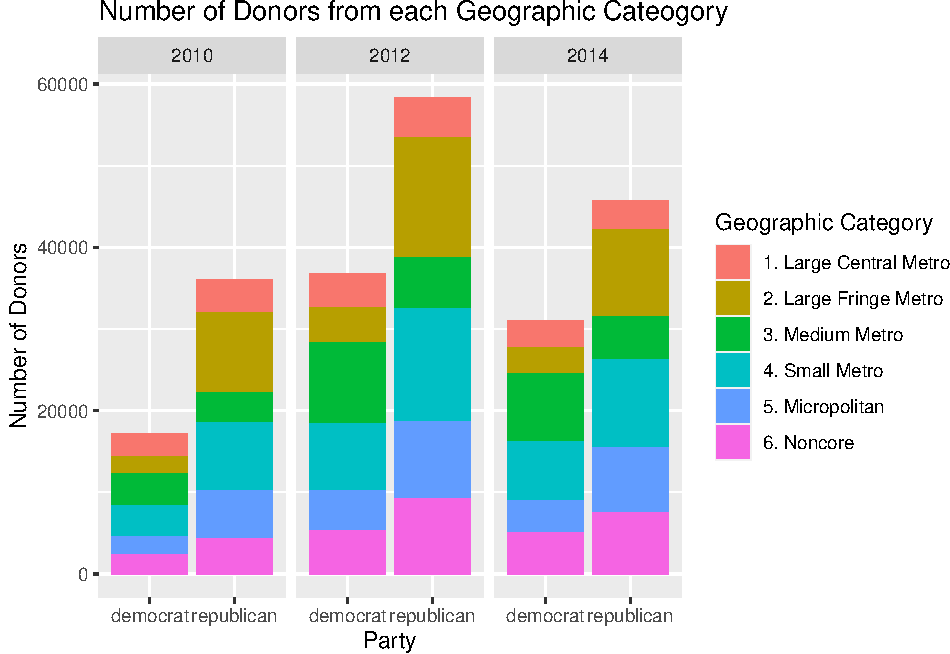
\includegraphics{scratch_files/figure-latex/unnamed-chunk-34-1.pdf}
\newpage

\begin{longtable}[]{@{}llrll@{}}
\caption{Bootstrapped difference-in-means test with 1,000 replications
comparing mean partisanship by geographic category.}\tabularnewline
\toprule
Geographic Category & Election Year & Diff. & CI & p\tabularnewline
\midrule
\endfirsthead
\toprule
Geographic Category & Election Year & Diff. & CI & p\tabularnewline
\midrule
\endhead
1. Large Central Metro & 2012 compared to 2010 & 0.02168 &
0.01738-0.02596 & \textless.001\tabularnewline
2. Large Fringe Metro & 2012 compared to 2010 & 0.02665 & 0.02354-0.0301
& \textless.001\tabularnewline
3. Medium Metro & 2012 compared to 2010 & 0.04829 & 0.04328-0.05292 &
\textless.001\tabularnewline
4. Small Metro & 2012 compared to 2010 & 0.03639 & 0.0331-0.03996 &
\textless.001\tabularnewline
5. Micropolitan & 2012 compared to 2010 & 0.03165 & 0.02764-0.03597 &
\textless.001\tabularnewline
6. Noncore & 2012 compared to 2010 & 0.04219 & 0.03748-0.04716 &
\textless.001\tabularnewline
1. Large Central Metro & 2014 compared to 2012 & 0.00296 &
0.00023-0.00569 & 0.03\tabularnewline
2. Large Fringe Metro & 2014 compared to 2012 & 0.00553 & 0.0037-0.00736
& \textless.001\tabularnewline
3. Medium Metro & 2014 compared to 2012 & -0.00184 & -0.0043-0.00064 &
0.128\tabularnewline
4. Small Metro & 2014 compared to 2012 & -0.00029 & -0.00216-0.00154 &
0.78\tabularnewline
5. Micropolitan & 2014 compared to 2012 & 0.00104 & -0.00106-0.00312 &
0.36\tabularnewline
6. Noncore & 2014 compared to 2012 & -0.00086 & -0.00305-0.00131 &
0.414\tabularnewline
\bottomrule
\end{longtable}

I ran the same bootstrapping test on the donor data based on the NCHS
scheme and saw that in 2014, both urban areas got significantly more
polarized. This disagrees with the rucc scheme, which showed that
Madison and Milwaukee did not get significantly more polarized in 2014.
I decided to pull the cities from the ``Large Fringe'' group and found
that they were a subset of the ``2. Urban: Not Madison and Milwaukee''
category.

The results of further testing by party are below:

\begin{longtable}[]{@{}lllrll@{}}
\caption{Bootstrapped difference-in-means test with 1,000 replications
comparing mean partisanship by geographic category.}\tabularnewline
\toprule
\begin{minipage}[b]{0.22\columnwidth}\raggedright
Geographic Category\strut
\end{minipage} & \begin{minipage}[b]{0.10\columnwidth}\raggedright
Party\strut
\end{minipage} & \begin{minipage}[b]{0.21\columnwidth}\raggedright
Election Year\strut
\end{minipage} & \begin{minipage}[b]{0.09\columnwidth}\raggedleft
Diff.\strut
\end{minipage} & \begin{minipage}[b]{0.16\columnwidth}\raggedright
CI\strut
\end{minipage} & \begin{minipage}[b]{0.06\columnwidth}\raggedright
p\strut
\end{minipage}\tabularnewline
\midrule
\endfirsthead
\toprule
\begin{minipage}[b]{0.22\columnwidth}\raggedright
Geographic Category\strut
\end{minipage} & \begin{minipage}[b]{0.10\columnwidth}\raggedright
Party\strut
\end{minipage} & \begin{minipage}[b]{0.21\columnwidth}\raggedright
Election Year\strut
\end{minipage} & \begin{minipage}[b]{0.09\columnwidth}\raggedleft
Diff.\strut
\end{minipage} & \begin{minipage}[b]{0.16\columnwidth}\raggedright
CI\strut
\end{minipage} & \begin{minipage}[b]{0.06\columnwidth}\raggedright
p\strut
\end{minipage}\tabularnewline
\midrule
\endhead
\begin{minipage}[t]{0.22\columnwidth}\raggedright
1. Large Central Metro\strut
\end{minipage} & \begin{minipage}[t]{0.10\columnwidth}\raggedright
democrat\strut
\end{minipage} & \begin{minipage}[t]{0.21\columnwidth}\raggedright
2012 compared to 2010\strut
\end{minipage} & \begin{minipage}[t]{0.09\columnwidth}\raggedleft
0.02653\strut
\end{minipage} & \begin{minipage}[t]{0.16\columnwidth}\raggedright
0.0208-0.03291\strut
\end{minipage} & \begin{minipage}[t]{0.06\columnwidth}\raggedright
\textless.001\strut
\end{minipage}\tabularnewline
\begin{minipage}[t]{0.22\columnwidth}\raggedright
2. Large Fringe Metro\strut
\end{minipage} & \begin{minipage}[t]{0.10\columnwidth}\raggedright
democrat\strut
\end{minipage} & \begin{minipage}[t]{0.21\columnwidth}\raggedright
2012 compared to 2010\strut
\end{minipage} & \begin{minipage}[t]{0.09\columnwidth}\raggedleft
0.05834\strut
\end{minipage} & \begin{minipage}[t]{0.16\columnwidth}\raggedright
0.04825-0.06895\strut
\end{minipage} & \begin{minipage}[t]{0.06\columnwidth}\raggedright
\textless.001\strut
\end{minipage}\tabularnewline
\begin{minipage}[t]{0.22\columnwidth}\raggedright
3. Medium Metro\strut
\end{minipage} & \begin{minipage}[t]{0.10\columnwidth}\raggedright
democrat\strut
\end{minipage} & \begin{minipage}[t]{0.21\columnwidth}\raggedright
2012 compared to 2010\strut
\end{minipage} & \begin{minipage}[t]{0.09\columnwidth}\raggedleft
0.03955\strut
\end{minipage} & \begin{minipage}[t]{0.16\columnwidth}\raggedright
0.03444-0.04505\strut
\end{minipage} & \begin{minipage}[t]{0.06\columnwidth}\raggedright
\textless.001\strut
\end{minipage}\tabularnewline
\begin{minipage}[t]{0.22\columnwidth}\raggedright
4. Small Metro\strut
\end{minipage} & \begin{minipage}[t]{0.10\columnwidth}\raggedright
democrat\strut
\end{minipage} & \begin{minipage}[t]{0.21\columnwidth}\raggedright
2012 compared to 2010\strut
\end{minipage} & \begin{minipage}[t]{0.09\columnwidth}\raggedleft
0.04310\strut
\end{minipage} & \begin{minipage}[t]{0.16\columnwidth}\raggedright
0.03718-0.04948\strut
\end{minipage} & \begin{minipage}[t]{0.06\columnwidth}\raggedright
\textless.001\strut
\end{minipage}\tabularnewline
\begin{minipage}[t]{0.22\columnwidth}\raggedright
5. Micropolitan\strut
\end{minipage} & \begin{minipage}[t]{0.10\columnwidth}\raggedright
democrat\strut
\end{minipage} & \begin{minipage}[t]{0.21\columnwidth}\raggedright
2012 compared to 2010\strut
\end{minipage} & \begin{minipage}[t]{0.09\columnwidth}\raggedleft
0.04262\strut
\end{minipage} & \begin{minipage}[t]{0.16\columnwidth}\raggedright
0.03543-0.05026\strut
\end{minipage} & \begin{minipage}[t]{0.06\columnwidth}\raggedright
\textless.001\strut
\end{minipage}\tabularnewline
\begin{minipage}[t]{0.22\columnwidth}\raggedright
6. Noncore\strut
\end{minipage} & \begin{minipage}[t]{0.10\columnwidth}\raggedright
democrat\strut
\end{minipage} & \begin{minipage}[t]{0.21\columnwidth}\raggedright
2012 compared to 2010\strut
\end{minipage} & \begin{minipage}[t]{0.09\columnwidth}\raggedleft
0.04626\strut
\end{minipage} & \begin{minipage}[t]{0.16\columnwidth}\raggedright
0.0389-0.05397\strut
\end{minipage} & \begin{minipage}[t]{0.06\columnwidth}\raggedright
\textless.001\strut
\end{minipage}\tabularnewline
\begin{minipage}[t]{0.22\columnwidth}\raggedright
1. Large Central Metro\strut
\end{minipage} & \begin{minipage}[t]{0.10\columnwidth}\raggedright
democrat\strut
\end{minipage} & \begin{minipage}[t]{0.21\columnwidth}\raggedright
2014 compared to 2012\strut
\end{minipage} & \begin{minipage}[t]{0.09\columnwidth}\raggedleft
0.00185\strut
\end{minipage} & \begin{minipage}[t]{0.16\columnwidth}\raggedright
-0.00158-0.00512\strut
\end{minipage} & \begin{minipage}[t]{0.06\columnwidth}\raggedright
0.26\strut
\end{minipage}\tabularnewline
\begin{minipage}[t]{0.22\columnwidth}\raggedright
2. Large Fringe Metro\strut
\end{minipage} & \begin{minipage}[t]{0.10\columnwidth}\raggedright
democrat\strut
\end{minipage} & \begin{minipage}[t]{0.21\columnwidth}\raggedright
2014 compared to 2012\strut
\end{minipage} & \begin{minipage}[t]{0.09\columnwidth}\raggedleft
0.01416\strut
\end{minipage} & \begin{minipage}[t]{0.16\columnwidth}\raggedright
0.00934-0.01883\strut
\end{minipage} & \begin{minipage}[t]{0.06\columnwidth}\raggedright
\textless.001\strut
\end{minipage}\tabularnewline
\begin{minipage}[t]{0.22\columnwidth}\raggedright
3. Medium Metro\strut
\end{minipage} & \begin{minipage}[t]{0.10\columnwidth}\raggedright
democrat\strut
\end{minipage} & \begin{minipage}[t]{0.21\columnwidth}\raggedright
2014 compared to 2012\strut
\end{minipage} & \begin{minipage}[t]{0.09\columnwidth}\raggedleft
0.00070\strut
\end{minipage} & \begin{minipage}[t]{0.16\columnwidth}\raggedright
-0.00148-0.00286\strut
\end{minipage} & \begin{minipage}[t]{0.06\columnwidth}\raggedright
0.518\strut
\end{minipage}\tabularnewline
\begin{minipage}[t]{0.22\columnwidth}\raggedright
4. Small Metro\strut
\end{minipage} & \begin{minipage}[t]{0.10\columnwidth}\raggedright
democrat\strut
\end{minipage} & \begin{minipage}[t]{0.21\columnwidth}\raggedright
2014 compared to 2012\strut
\end{minipage} & \begin{minipage}[t]{0.09\columnwidth}\raggedleft
0.00130\strut
\end{minipage} & \begin{minipage}[t]{0.16\columnwidth}\raggedright
-0.00141-0.00393\strut
\end{minipage} & \begin{minipage}[t]{0.06\columnwidth}\raggedright
0.336\strut
\end{minipage}\tabularnewline
\begin{minipage}[t]{0.22\columnwidth}\raggedright
5. Micropolitan\strut
\end{minipage} & \begin{minipage}[t]{0.10\columnwidth}\raggedright
democrat\strut
\end{minipage} & \begin{minipage}[t]{0.21\columnwidth}\raggedright
2014 compared to 2012\strut
\end{minipage} & \begin{minipage}[t]{0.09\columnwidth}\raggedleft
0.00141\strut
\end{minipage} & \begin{minipage}[t]{0.16\columnwidth}\raggedright
-0.00159-0.00462\strut
\end{minipage} & \begin{minipage}[t]{0.06\columnwidth}\raggedright
0.372\strut
\end{minipage}\tabularnewline
\begin{minipage}[t]{0.22\columnwidth}\raggedright
6. Noncore\strut
\end{minipage} & \begin{minipage}[t]{0.10\columnwidth}\raggedright
democrat\strut
\end{minipage} & \begin{minipage}[t]{0.21\columnwidth}\raggedright
2014 compared to 2012\strut
\end{minipage} & \begin{minipage}[t]{0.09\columnwidth}\raggedleft
-0.00238\strut
\end{minipage} & \begin{minipage}[t]{0.16\columnwidth}\raggedright
-0.00509-0.00044\strut
\end{minipage} & \begin{minipage}[t]{0.06\columnwidth}\raggedright
0.108\strut
\end{minipage}\tabularnewline
\begin{minipage}[t]{0.22\columnwidth}\raggedright
1. Large Central Metro\strut
\end{minipage} & \begin{minipage}[t]{0.10\columnwidth}\raggedright
republican\strut
\end{minipage} & \begin{minipage}[t]{0.21\columnwidth}\raggedright
2012 compared to 2010\strut
\end{minipage} & \begin{minipage}[t]{0.09\columnwidth}\raggedleft
0.00954\strut
\end{minipage} & \begin{minipage}[t]{0.16\columnwidth}\raggedright
0.00525-0.01425\strut
\end{minipage} & \begin{minipage}[t]{0.06\columnwidth}\raggedright
\textless.001\strut
\end{minipage}\tabularnewline
\begin{minipage}[t]{0.22\columnwidth}\raggedright
2. Large Fringe Metro\strut
\end{minipage} & \begin{minipage}[t]{0.10\columnwidth}\raggedright
republican\strut
\end{minipage} & \begin{minipage}[t]{0.21\columnwidth}\raggedright
2012 compared to 2010\strut
\end{minipage} & \begin{minipage}[t]{0.09\columnwidth}\raggedleft
0.01411\strut
\end{minipage} & \begin{minipage}[t]{0.16\columnwidth}\raggedright
0.01152-0.01676\strut
\end{minipage} & \begin{minipage}[t]{0.06\columnwidth}\raggedright
\textless.001\strut
\end{minipage}\tabularnewline
\begin{minipage}[t]{0.22\columnwidth}\raggedright
3. Medium Metro\strut
\end{minipage} & \begin{minipage}[t]{0.10\columnwidth}\raggedright
republican\strut
\end{minipage} & \begin{minipage}[t]{0.21\columnwidth}\raggedright
2012 compared to 2010\strut
\end{minipage} & \begin{minipage}[t]{0.09\columnwidth}\raggedleft
0.04315\strut
\end{minipage} & \begin{minipage}[t]{0.16\columnwidth}\raggedright
0.03664-0.04941\strut
\end{minipage} & \begin{minipage}[t]{0.06\columnwidth}\raggedright
\textless.001\strut
\end{minipage}\tabularnewline
\begin{minipage}[t]{0.22\columnwidth}\raggedright
4. Small Metro\strut
\end{minipage} & \begin{minipage}[t]{0.10\columnwidth}\raggedright
republican\strut
\end{minipage} & \begin{minipage}[t]{0.21\columnwidth}\raggedright
2012 compared to 2010\strut
\end{minipage} & \begin{minipage}[t]{0.09\columnwidth}\raggedleft
0.02344\strut
\end{minipage} & \begin{minipage}[t]{0.16\columnwidth}\raggedright
0.02018-0.02692\strut
\end{minipage} & \begin{minipage}[t]{0.06\columnwidth}\raggedright
\textless.001\strut
\end{minipage}\tabularnewline
\begin{minipage}[t]{0.22\columnwidth}\raggedright
5. Micropolitan\strut
\end{minipage} & \begin{minipage}[t]{0.10\columnwidth}\raggedright
republican\strut
\end{minipage} & \begin{minipage}[t]{0.21\columnwidth}\raggedright
2012 compared to 2010\strut
\end{minipage} & \begin{minipage}[t]{0.09\columnwidth}\raggedleft
0.01960\strut
\end{minipage} & \begin{minipage}[t]{0.16\columnwidth}\raggedright
0.01587-0.02343\strut
\end{minipage} & \begin{minipage}[t]{0.06\columnwidth}\raggedright
\textless.001\strut
\end{minipage}\tabularnewline
\begin{minipage}[t]{0.22\columnwidth}\raggedright
6. Noncore\strut
\end{minipage} & \begin{minipage}[t]{0.10\columnwidth}\raggedright
republican\strut
\end{minipage} & \begin{minipage}[t]{0.21\columnwidth}\raggedright
2012 compared to 2010\strut
\end{minipage} & \begin{minipage}[t]{0.09\columnwidth}\raggedleft
0.02602\strut
\end{minipage} & \begin{minipage}[t]{0.16\columnwidth}\raggedright
0.02145-0.03014\strut
\end{minipage} & \begin{minipage}[t]{0.06\columnwidth}\raggedright
\textless.001\strut
\end{minipage}\tabularnewline
\begin{minipage}[t]{0.22\columnwidth}\raggedright
1. Large Central Metro\strut
\end{minipage} & \begin{minipage}[t]{0.10\columnwidth}\raggedright
republican\strut
\end{minipage} & \begin{minipage}[t]{0.21\columnwidth}\raggedright
2014 compared to 2012\strut
\end{minipage} & \begin{minipage}[t]{0.09\columnwidth}\raggedleft
0.00274\strut
\end{minipage} & \begin{minipage}[t]{0.16\columnwidth}\raggedright
-0.00071-0.00613\strut
\end{minipage} & \begin{minipage}[t]{0.06\columnwidth}\raggedright
0.114\strut
\end{minipage}\tabularnewline
\begin{minipage}[t]{0.22\columnwidth}\raggedright
2. Large Fringe Metro\strut
\end{minipage} & \begin{minipage}[t]{0.10\columnwidth}\raggedright
republican\strut
\end{minipage} & \begin{minipage}[t]{0.21\columnwidth}\raggedright
2014 compared to 2012\strut
\end{minipage} & \begin{minipage}[t]{0.09\columnwidth}\raggedleft
0.00242\strut
\end{minipage} & \begin{minipage}[t]{0.16\columnwidth}\raggedright
0.00089-0.00395\strut
\end{minipage} & \begin{minipage}[t]{0.06\columnwidth}\raggedright
0.002\strut
\end{minipage}\tabularnewline
\begin{minipage}[t]{0.22\columnwidth}\raggedright
3. Medium Metro\strut
\end{minipage} & \begin{minipage}[t]{0.10\columnwidth}\raggedright
republican\strut
\end{minipage} & \begin{minipage}[t]{0.21\columnwidth}\raggedright
2014 compared to 2012\strut
\end{minipage} & \begin{minipage}[t]{0.09\columnwidth}\raggedleft
-0.00545\strut
\end{minipage} & \begin{minipage}[t]{0.16\columnwidth}\raggedright
-0.0095--0.00121\strut
\end{minipage} & \begin{minipage}[t]{0.06\columnwidth}\raggedright
0.01\strut
\end{minipage}\tabularnewline
\begin{minipage}[t]{0.22\columnwidth}\raggedright
4. Small Metro\strut
\end{minipage} & \begin{minipage}[t]{0.10\columnwidth}\raggedright
republican\strut
\end{minipage} & \begin{minipage}[t]{0.21\columnwidth}\raggedright
2014 compared to 2012\strut
\end{minipage} & \begin{minipage}[t]{0.09\columnwidth}\raggedleft
-0.00183\strut
\end{minipage} & \begin{minipage}[t]{0.16\columnwidth}\raggedright
-0.00392-0.00016\strut
\end{minipage} & \begin{minipage}[t]{0.06\columnwidth}\raggedright
0.076\strut
\end{minipage}\tabularnewline
\begin{minipage}[t]{0.22\columnwidth}\raggedright
5. Micropolitan\strut
\end{minipage} & \begin{minipage}[t]{0.10\columnwidth}\raggedright
republican\strut
\end{minipage} & \begin{minipage}[t]{0.21\columnwidth}\raggedright
2014 compared to 2012\strut
\end{minipage} & \begin{minipage}[t]{0.09\columnwidth}\raggedleft
0.00157\strut
\end{minipage} & \begin{minipage}[t]{0.16\columnwidth}\raggedright
-5e-04-0.00385\strut
\end{minipage} & \begin{minipage}[t]{0.06\columnwidth}\raggedright
0.15\strut
\end{minipage}\tabularnewline
\begin{minipage}[t]{0.22\columnwidth}\raggedright
6. Noncore\strut
\end{minipage} & \begin{minipage}[t]{0.10\columnwidth}\raggedright
republican\strut
\end{minipage} & \begin{minipage}[t]{0.21\columnwidth}\raggedright
2014 compared to 2012\strut
\end{minipage} & \begin{minipage}[t]{0.09\columnwidth}\raggedleft
-0.00072\strut
\end{minipage} & \begin{minipage}[t]{0.16\columnwidth}\raggedright
-0.00292-0.00134\strut
\end{minipage} & \begin{minipage}[t]{0.06\columnwidth}\raggedright
0.524\strut
\end{minipage}\tabularnewline
\bottomrule
\end{longtable}

\begin{verbatim}
## Warning: Removed 1 rows containing missing values (geom_errorbarh).
\end{verbatim}

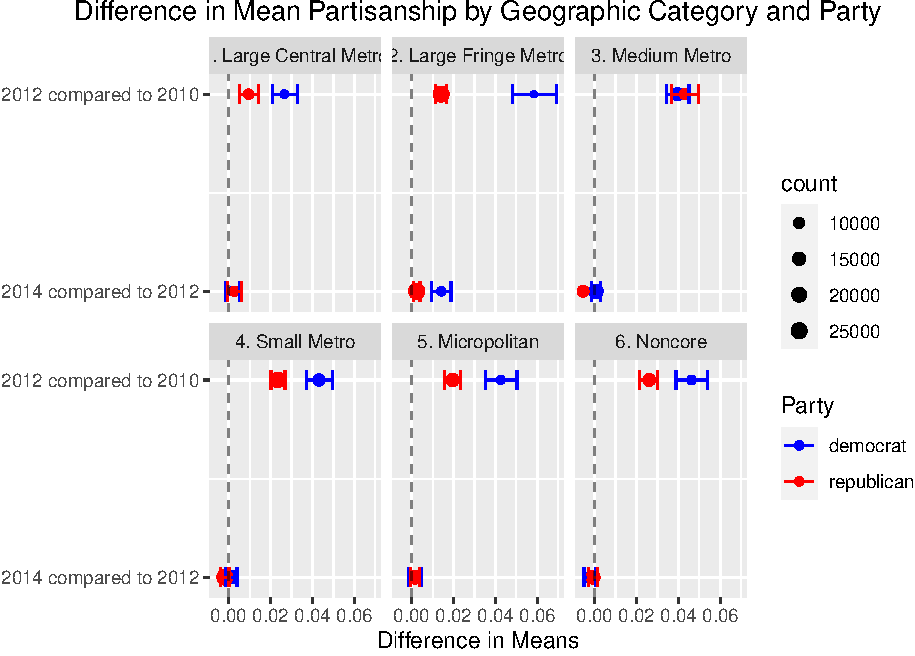
\includegraphics{scratch_files/figure-latex/unnamed-chunk-39-1.pdf}
\newpage

\hypertarget{rural-urban-commuting-area-codes-rucas}{%
\subsubsection{Rural-Urban Commuting Area Codes
(RUCAs)}\label{rural-urban-commuting-area-codes-rucas}}

From \url{https://depts.washington.edu/uwruca/index.php}

``RUCAs, Rural-Urban Commuting Area Codes, are a new Census tract-based
classification scheme that utilizes the standard Bureau of Census
Urbanized Area and Urban Cluster definitions in combination with work
commuting information to characterize all of the nation's Census tracts
regarding their rural and urban status and relationships. In addition, a
ZIP Code RUCA approximation was developed.''

Documentation for variables:
\url{https://depts.washington.edu/uwruca/ruca-documentation.php}

UA=Urbanized Area UC=Urban Cluster

\begin{longtable}[]{@{}ll@{}}
\caption{Rural-Urban Commuting Area Codes}\tabularnewline
\toprule
\begin{minipage}[b]{0.08\columnwidth}\raggedright
RUCA Code\strut
\end{minipage} & \begin{minipage}[b]{0.86\columnwidth}\raggedright
Description\strut
\end{minipage}\tabularnewline
\midrule
\endfirsthead
\toprule
\begin{minipage}[b]{0.08\columnwidth}\raggedright
RUCA Code\strut
\end{minipage} & \begin{minipage}[b]{0.86\columnwidth}\raggedright
Description\strut
\end{minipage}\tabularnewline
\midrule
\endhead
\begin{minipage}[t]{0.08\columnwidth}\raggedright
1\strut
\end{minipage} & \begin{minipage}[t]{0.86\columnwidth}\raggedright
Metropolitan area core: primary flow within an Urbanized Area (UA)\strut
\end{minipage}\tabularnewline
\begin{minipage}[t]{0.08\columnwidth}\raggedright
2\strut
\end{minipage} & \begin{minipage}[t]{0.86\columnwidth}\raggedright
Metropolitan area high commuting: primary flow 30\% or more to a
UA\strut
\end{minipage}\tabularnewline
\begin{minipage}[t]{0.08\columnwidth}\raggedright
3\strut
\end{minipage} & \begin{minipage}[t]{0.86\columnwidth}\raggedright
Metropolitan area low commuting: primary flow 10\% to 30\% to a UA\strut
\end{minipage}\tabularnewline
\begin{minipage}[t]{0.08\columnwidth}\raggedright
4\strut
\end{minipage} & \begin{minipage}[t]{0.86\columnwidth}\raggedright
Micropolitan* area core: primary flow within an Urban Cluster (UC) of
10,000 through 49,999 (large UC)\strut
\end{minipage}\tabularnewline
\begin{minipage}[t]{0.08\columnwidth}\raggedright
5\strut
\end{minipage} & \begin{minipage}[t]{0.86\columnwidth}\raggedright
Micropolitan* high commuting: primary flow 30\% or more to a large
UC\strut
\end{minipage}\tabularnewline
\begin{minipage}[t]{0.08\columnwidth}\raggedright
6\strut
\end{minipage} & \begin{minipage}[t]{0.86\columnwidth}\raggedright
Micropolitan* low commuting: primary flow 10\% to 30\% to a large
UC\strut
\end{minipage}\tabularnewline
\begin{minipage}[t]{0.08\columnwidth}\raggedright
7\strut
\end{minipage} & \begin{minipage}[t]{0.86\columnwidth}\raggedright
Small town core: primary flow within an Urban Cluster of 2,500 through
9,999 (small UC)\strut
\end{minipage}\tabularnewline
\begin{minipage}[t]{0.08\columnwidth}\raggedright
8\strut
\end{minipage} & \begin{minipage}[t]{0.86\columnwidth}\raggedright
Small town high commuting: primary flow 30\% or more to a small UC\strut
\end{minipage}\tabularnewline
\begin{minipage}[t]{0.08\columnwidth}\raggedright
9\strut
\end{minipage} & \begin{minipage}[t]{0.86\columnwidth}\raggedright
Small town low commuting: primary flow 10\% through 29\% to a small
UC\strut
\end{minipage}\tabularnewline
\begin{minipage}[t]{0.08\columnwidth}\raggedright
10\strut
\end{minipage} & \begin{minipage}[t]{0.86\columnwidth}\raggedright
Rural areas: primary flow to a tract outside a UA or UC (including
self)\strut
\end{minipage}\tabularnewline
\bottomrule
\end{longtable}

Each category had a couple of subcategories (7, 7.1, 7.2, etc) to
further break down the categories but I simplified it just by taking the
floor of the full code (everything rounds down).

\begin{longtable}[]{@{}llrll@{}}
\caption{Bootstrapped difference-in-means test with 1,000 replications
comparing mean partisanship by geographic category.}\tabularnewline
\toprule
Geographic Category & Election Year & Diff. & CI & p\tabularnewline
\midrule
\endfirsthead
\toprule
Geographic Category & Election Year & Diff. & CI & p\tabularnewline
\midrule
\endhead
1 & 2012 compared to 2010 & 0.03481 & 0.0326-0.03706 &
\textless.001\tabularnewline
2 & 2012 compared to 2010 & 0.03435 & 0.02949-0.03882 &
\textless.001\tabularnewline
3 & 2012 compared to 2010 & 0.04381 & 0.0241-0.06418 &
\textless.001\tabularnewline
4 & 2012 compared to 2010 & 0.02445 & 0.01978-0.02935 &
\textless.001\tabularnewline
5 & 2012 compared to 2010 & 0.03794 & 0.02101-0.05562 &
\textless.001\tabularnewline
6 & 2012 compared to 2010 & 0.03123 & 0.01354-0.05087 &
\textless.001\tabularnewline
7 & 2012 compared to 2010 & 0.03672 & 0.03162-0.04207 &
\textless.001\tabularnewline
8 & 2012 compared to 2010 & 0.06756 & 0.04518-0.09145 &
\textless.001\tabularnewline
9 & 2012 compared to 2010 & 0.01166 & 0.00118-0.02443 &
0.034\tabularnewline
10 & 2012 compared to 2010 & 0.03217 & 0.02744-0.0372 &
\textless.001\tabularnewline
1 & 2014 compared to 2012 & 0.00017 & -0.00107-0.00136 &
0.798\tabularnewline
2 & 2014 compared to 2012 & 0.00117 & -0.00132-0.00348 &
0.354\tabularnewline
3 & 2014 compared to 2012 & -0.00331 & -0.01119-0.00412 &
0.386\tabularnewline
4 & 2014 compared to 2012 & 0.00613 & 0.00327-0.00924 &
\textless.001\tabularnewline
5 & 2014 compared to 2012 & -0.00254 & -0.01013-0.00471 &
0.478\tabularnewline
6 & 2014 compared to 2012 & -0.00141 & -0.01078-0.00741 &
0.776\tabularnewline
7 & 2014 compared to 2012 & 0.00405 & 0.00134-0.00691 &
\textless.001\tabularnewline
8 & 2014 compared to 2012 & 0.00123 & -0.00592-0.0087 &
0.74\tabularnewline
9 & 2014 compared to 2012 & 0.00070 & -0.00498-0.0068 &
0.794\tabularnewline
10 & 2014 compared to 2012 & -0.00247 & -0.00489--3e-05 &
0.046\tabularnewline
\bottomrule
\end{longtable}

\hypertarget{the-divided-but-not-more-predictable-electorate-a-machine-learning-analysis-of-voting-in-american-presidential-election}{%
\subsection{The Divided (But Not More Predictable) Electorate: A Machine
Learning Analysis of Voting in American Presidential
Election}\label{the-divided-but-not-more-predictable-electorate-a-machine-learning-analysis-of-voting-in-american-presidential-election}}

\url{https://preprints.apsanet.org/engage/api-gateway/apsa/assets/orp/resource/item/6050dba7df04091d6a7fb4ef/original/the-divided-but-not-more-predictable-electorate-a-machine-learning-analysis-of-voting-in-american-presidential-elections.pdf}

\begin{verbatim}
- Demographics have not become more predictive of vote choice
    - When all variables are included and some sort of stepping is performed, demographics do not make it into top 10 predictors
- Focus on 5 demographic markers: race, education, income, age, gender
\end{verbatim}

Main method used: random forests to predict voting predictions, using
data from five surveys - Also a logistic regression for voice choice as
y-variable, and CART model to confirm results

General results: demographics alone is a bad predictor (65\% ish or
less)





\newpage
\singlespacing 
\end{document}
